%%% The main file. It contains definitions of basic parameters and includes all other parts.

%% Settings for single-side (simplex) printing
% Margins: left 40mm, right 25mm, top and bottom 25mm
% (but beware, LaTeX adds 1in implicitly)
\documentclass[12pt,a4paper]{report}
\setlength\textwidth{145mm}
\setlength\textheight{247mm}
\setlength\oddsidemargin{15mm}
\setlength\evensidemargin{15mm}
\setlength\topmargin{0mm}
\setlength\headsep{0mm}
\setlength\headheight{0mm}
% \openright makes the following text appear on a right-hand page
\let\openright=\clearpage

%% Settings for two-sided (duplex) printing
% \documentclass[12pt,a4paper,twoside,openright]{report}
% \setlength\textwidth{145mm}
% \setlength\textheight{247mm}
% \setlength\oddsidemargin{14.2mm}
% \setlength\evensidemargin{0mm}
% \setlength\topmargin{0mm}
% \setlength\headsep{0mm}
% \setlength\headheight{0mm}
% \let\openright=\cleardoublepage

%% Generate PDF/A-2u
\usepackage[a-2u]{pdfx}

%% Character encoding: usually latin2, cp1250 or utf8:
\usepackage[utf8]{inputenc}

%% Prefer Latin Modern fonts
\usepackage{lmodern}

%% Further useful packages (included in most LaTeX distributions)
\usepackage{amsmath}        % extensions for typesetting of math
\usepackage{amsfonts}       % math fonts
\usepackage{amsthm}         % theorems, definitions, etc.
\usepackage{bbding}         % various symbols (squares, asterisks, scissors, ...)
\usepackage{bm}             % boldface symbols (\bm)
\usepackage{graphicx}       % embedding of pictures
\usepackage{fancyvrb}       % improved verbatim environment
\usepackage{natbib}         % citation style AUTHOR (YEAR), or AUTHOR [NUMBER]
\usepackage[nottoc]{tocbibind} % makes sure that bibliography and the lists
			    % of figures/tables are included in the table
			    % of contents
\usepackage{dcolumn}        % improved alignment of table columns
\usepackage{booktabs}       % improved horizontal lines in tables
\usepackage{paralist}       % improved enumerate and itemize
\usepackage{xcolor}         % typesetting in color

%% SPECIMEN
% Parts marked as SPECIMEN are used for building the example PDF.
% When the official template is generated by ./mkdist, all such parts
% are deleted, as well as all calls of \X and \XXX macros.
\def\X#1{\textcolor{red}{[#1]}}
\def\XXX#1{\par\smallskip\noindent \textcolor{red}{[#1]}}
%% NEMICEPS

%%% Basic information on the thesis

% Thesis title in English (exactly as in the formal assignment)
\def\ThesisTitle{Optical Music Recognition using Deep Neural Networks}

% Author of the thesis
\def\ThesisAuthor{Jiří Mayer}

% Year when the thesis is submitted
\def\YearSubmitted{2020}

% Name of the department or institute, where the work was officially assigned
% (according to the Organizational Structure of MFF UK in English,
% or a full name of a department outside MFF)
\def\Department{Institute of Formal and Applied Linguistics}

% Is it a department (katedra), or an institute (ústav)?
\def\DeptType{Department}

% Thesis supervisor: name, surname and titles
\def\Supervisor{doc. RNDr. Pavel Pecina, Ph.D.}

% Supervisor's department (again according to Organizational structure of MFF)
\def\SupervisorsDepartment{Institute of Formal and Applied Linguistics}

% Study programme and specialization
\def\StudyProgramme{Computer Science} % Informatika (B1801)
\def\StudyBranch{General Computer Science} % Obecná informatika IOI (1801R008)

% An optional dedication: you can thank whomever you wish (your supervisor,
% consultant, a person who lent the software, etc.)
\def\Dedication{%
Dedication.
}

% Abstract (recommended length around 80-200 words; this is not a copy of your thesis assignment!)
\def\Abstract{%
Optical music recognition is a~challenging field similar in many ways to optical text recognition. It~brings, however, many challenges that traditional pipeline-based recognition systems struggle with. The~end-to-end approach has proven to be superior in the domain of handwritten text recognition. We tried to apply this approach to the field of OMR. Specifically, we focused on handwritten music recognition. To resolve the lack of training data, we developed an engraving system for handwritten music called Mashcima. This engraving system is successful at mimicking the style of the CVC-MUSCIMA dataset. We evaluated our model on a~portion of the CVC-MUSCIMA dataset and the approach seems to be promising.
}

% 3 to 5 keywords (recommended), each enclosed in curly braces
\def\Keywords{%
{optical music recognition}, {handwritten music recognition}, {deep neural network}
}

%% The hyperref package for clickable links in PDF and also for storing
%% metadata to PDF (including the table of contents).
%% Most settings are pre-set by the pdfx package.
\hypersetup{unicode}
\hypersetup{breaklinks=true}

% Definitions of macros (see description inside)
%%% This file contains definitions of various useful macros and environments %%%
%%% Please add more macros here instead of cluttering other files with them. %%%

%%% Minor tweaks of style

% These macros employ a little dirty trick to convince LaTeX to typeset
% chapter headings sanely, without lots of empty space above them.
% Feel free to ignore.
\makeatletter
\def\@makechapterhead#1{
  {\parindent \z@ \raggedright \normalfont
   \Huge\bfseries \thechapter. #1
   \par\nobreak
   \vskip 20\p@
}}
\def\@makeschapterhead#1{
  {\parindent \z@ \raggedright \normalfont
   \Huge\bfseries #1
   \par\nobreak
   \vskip 20\p@
}}
\makeatother

% This macro defines a chapter, which is not numbered, but is included
% in the table of contents.
\def\chapwithtoc#1{
\chapter*{#1}
\addcontentsline{toc}{chapter}{#1}
}

% Draw black "slugs" whenever a line overflows, so that we can spot it easily.
\overfullrule=1mm

%%% Macros for definitions, theorems, claims, examples, ... (requires amsthm package)

\theoremstyle{plain}
\newtheorem{thm}{Theorem}
\newtheorem{lemma}[thm]{Lemma}
\newtheorem{claim}[thm]{Claim}

\theoremstyle{plain}
\newtheorem{defn}{Definition}

\theoremstyle{remark}
\newtheorem*{cor}{Corollary}
\newtheorem*{rem}{Remark}
\newtheorem*{example}{Example}

%%% An environment for proofs

\newenvironment{myproof}{
  \par\medskip\noindent
  \textit{Proof}.
}{
\newline
\rightline{$\qedsymbol$}
}

%%% An environment for typesetting of program code and input/output
%%% of programs. (Requires the fancyvrb package -- fancy verbatim.)

\DefineVerbatimEnvironment{code}{Verbatim}{fontsize=\small, frame=single}

%%% The field of all real and natural numbers
\newcommand{\R}{\mathbb{R}}
\newcommand{\N}{\mathbb{N}}

%%% Useful operators for statistics and probability
\DeclareMathOperator{\pr}{\textsf{P}}
\DeclareMathOperator{\E}{\textsf{E}\,}
\DeclareMathOperator{\var}{\textrm{var}}
\DeclareMathOperator{\sd}{\textrm{sd}}

%%% Transposition of a vector/matrix
\newcommand{\T}[1]{#1^\top}

%%% Various math goodies
\newcommand{\goto}{\rightarrow}
\newcommand{\gotop}{\stackrel{P}{\longrightarrow}}
\newcommand{\maon}[1]{o(n^{#1})}
\newcommand{\abs}[1]{\left|{#1}\right|}
\newcommand{\dint}{\int_0^\tau\!\!\int_0^\tau}
\newcommand{\isqr}[1]{\frac{1}{\sqrt{#1}}}

%%% Various table goodies
\newcommand{\pulrad}[1]{\raisebox{1.5ex}[0pt]{#1}}
\newcommand{\mc}[1]{\multicolumn{1}{c}{#1}}


% Title page and various mandatory informational pages
\begin{document}
%%% Title page of the thesis and other mandatory pages

%%% SPECIMEN
%%% Inscriptions at the opening page of the hard cover
\iffalse % disable the hard cover page

\pagestyle{empty}
\hypersetup{pageanchor=false}
\XXX{Opening page of the hard cover. Not a part of the electronic version.}
\begin{center}

\large
Charles University

\medskip

Faculty of Mathematics and Physics

\vfill

{\huge\bf BACHELOR THESIS}

\vfill

\hbox to \hsize{\YearSubmitted\hfil \ThesisAuthor}

\end{center}

\newpage\openright

\fi
%%% NEMICEPS

%%% Title page of the thesis

\pagestyle{empty}
\hypersetup{pageanchor=false}
\begin{center}

\centerline{\mbox{
\includegraphics[width=166mm]{../img/logo-en.pdf}}}

\vspace{-8mm}
\vfill

{\bf\Large BACHELOR THESIS}

\vfill

% SVOC competition - note on the submission
\noindent\rule{8cm}{0.4pt}\\
{\large\bf{This work is being submitted\\to the SVOČ 2021 competition}}\\
\noindent\rule{8cm}{0.4pt}
\vfill

{\LARGE\ThesisAuthor}

\vspace{15mm}

{\LARGE\bfseries\ThesisTitle}

\vfill

\Department

\vfill

{
\centerline{\vbox{\halign{\hbox to 0.45\hsize{\hfil #}&\hskip 0.5em\parbox[t]{0.45\hsize}{\raggedright #}\cr
Supervisor of the bachelor thesis:&\Supervisor \cr
\noalign{\vspace{2mm}}
Study programme:&\StudyProgramme \cr
\noalign{\vspace{2mm}}
Study branch:&\StudyBranch \cr
}}}}

\vfill

% Zde doplňte rok
Prague \YearSubmitted

\end{center}

\newpage

%%% NOPHD
%%% Here should be a bound sheet included -- a signed copy of the "bachelor
%%% thesis assignment". This assignment is NOT a part of the electronic
%%% version of the thesis. DO NOT SCAN.
\iffalse % hide the red text
\XXX{Bound into the introductory part must be the form with signed approval of the thesis topic (a photocopy suffices). This is not a~part of the electronic version of the thesis, do not scan!}
\fi
%%% PHDNO

%%% A page with a solemn declaration to the bachelor thesis

\openright
\hypersetup{pageanchor=true}
\pagestyle{plain}
\pagenumbering{roman}
\vglue 0pt plus 1fill

\noindent
I declare that I carried out this bachelor thesis independently, and only with the cited
sources, literature and other professional sources. It has not been used to obtain another
or the same degree.

\medskip\noindent
I understand that my work relates to the rights and obligations under the Act No.~121/2000 Sb.,
the Copyright Act, as amended, in particular the fact that the Charles
University has the right to conclude a license agreement on the use of this
work as a school work pursuant to Section 60 subsection 1 of the Copyright~Act.

\vspace{10mm}

\hbox{\hbox to 0.5\hsize{%
In \hbox to 6em{\dotfill} date \hbox to 6em{\dotfill}
\hss}\hbox to 0.5\hsize{\dotfill\quad}}
\smallskip
\hbox{\hbox to 0.5\hsize{}\hbox to 0.5\hsize{\hfil Author's signature\hfil}}

\vspace{20mm}
\newpage

%%% Dedication

\openright

\noindent
\Dedication

\newpage

%%% Mandatory information page of the thesis

\openright

\vbox to 0.5\vsize{
\setlength\parindent{0mm}
\setlength\parskip{5mm}

Title:
\ThesisTitle

Author:
\ThesisAuthor

\DeptType:
\Department

Supervisor:
\Supervisor, \SupervisorsDepartment

Abstract:
\Abstract

Keywords:
\Keywords

%\XXX{This information must be stored as PDF meta-data, too. Please refer to the {\tt README} file.}
\vss}

\newpage

\openright
\pagestyle{plain}
\pagenumbering{arabic}
\setcounter{page}{1}


%%% A page with automatically generated table of contents of the bachelor thesis

\tableofcontents

%%% Each chapter is kept in a separate file
\chapter{Introduction}
\label{chap:Introduction}

Optical music recognition (OMR) is an~interesting subfield of computer vision. It shares a~lot of similarities to optical character recognition (OCR) and handwritten text recognition (HTR). It is, however, more challenging as is pointed out in the~paper \emph{Understanding Optical Music Recognition} (\cite{CalvoZaragozaHajic}). For~example in OCR, characters are read in one direction, typically from left to right. Musical symbols seem to be similar in that a~staff is also read from left to right, but many symbols can be placed above each other. Piano scores can even have symbols that span multiple staves.

Although a~musical score can be very complex, many scores are not. We can limit ourselves to scores that are monophonic, have a~single voice, and have symbols spanning only one staff. Monophonic scores lack chords, meaning there's only one note playing at a~time. This holds, for example, for windblown instruments, since they cannot play multiple notes simultaneously. Sometimes multiple voices (instruments) are engraved in a~single staff to save space. We will not attempt to read these scores either. It would be like reading two lines of text simultaneously and the proposed model can output only a~single sequence. Also deciding what voice a~given note belongs to is in itself a~complicated problem.

Deep neural networks have transformed the field of computer vision recently. Especially convolutional networks (CNN), whose architecture is particularly well suited for image processing. Recurrent neural networks (RNN) have been used for sequence processing, like natural language modeling or natural language translation. We can combine these two architectures to create a~so-called RCNN network. When trained using connectionist temporal classification (CTC), we get a~powerful architecture that is ideal for processing visual sequential data (\cite{Puigcerver}). This architecture has been used in handwritten text recognition to yield state-of-the-art results (\cite{Scheidl}).

If we limit the~complexity of musical scores to the point that a~single staff can be represented as a~sequence of tokens, we can use this architecture to tackle the problem of OMR. This approach has been tried in 2018 by Calvo-Zaragoza and Rizo (\cite{Primus}). They created the PrIMuS dataset, which contains 87678 real-music incipits. An~incipit is the part of a~melody or a~musical work that is most recognizable for that work. Each incipit is a~few measures long, typically shorter than a~single staff of printed sheet music would be.

The resulting model has been compared against Audiveris\footnote{\href{https://github.com/Audiveris}{https://github.com/Audiveris}}, an~open-source OMR tool, and has proven to be superior on the~PrIMuS dataset. However, the~dataset contains printed images only. Since this RCNN architecture is an~end-to-end approach, there's a~great chance that it would be ideal for reading handwritten scores as~well (drawing analogy from HTR).

Therefore the goal of this thesis is to explore the~end-to-end approach for optical music recognition of handwritten music scores. More specifically we want to train an~RCNN network to yield the best possible results on the~CVC-MUSCIMA dataset.

\overfullrule=0pt % fixes black rectangle issue
We needed to obtain training data. We explored the \emph{Collection of datasets for OMR} by~Alexander Pacha (\cite{Pacha}) and quickly found out that the~only dataset containing entire staves of handwritten sheet music is the~CVC-MUSCIMA dataset (\cite{CvcMuscima}). Every other handwritten dataset contains only musical symbols or is derived from CVC-MUSCIMA. Since CVC-MUSCIMA is intended for writer classification and staff removal, it contains only 20 parts, each written by 50 writers. That's far too small variability, given the~task we are trying to solve.

Facing this issue we resorted to data augmentation. The~idea is to take handwritten musical symbols and place them onto an~empty staff to create a~new staff image. We called this music engraving system \emph{Mashcima} and the~system is explained in chapter \ref{chap:EngravingSystem}. The~musical symbols used by~Mashcima come from the~MUSCIMA++ dataset (\cite{MuscimaPP}). This~dataset is built on top of CVC-MUSCIMA and provides pixel-perfect symbol segmentation and relationships between symbols. The~reason we choose MUSCIMA++, instead of other musical symbol datasets, is that it is built on top of CVC-MUSCIMA. This means the~image resolution and overall style are consistent with CVC-MUSCIMA. Also, MUSCIMA++ has been developed at~Charles University and~so it was easy to contact its creator when needed. We however do make sure, that the~final evaluation is performed on data the~neural network has not seen during training. Specifically, it trains on staves by completely different writers than the~ones used for evaluation.

Mashcima engraving system is the~main feature that sets this thesis apart from other works. Other people, when faced with the~lack of training data, used data augmentation (dilation, blurring, distortion) or transfer learning (\cite{HmrBaseline}). We believe that a~custom engraving system for handwritten music is the~best way to produce an~overabundance of high-quality training data. Our confidence stems from the fact, that non-trained human has difficulties distinguishing a~real-world sample from a~well-engraved one (see Figure \ref{fig1:Comparison}).

\begin{figure}[h]
    \centering
    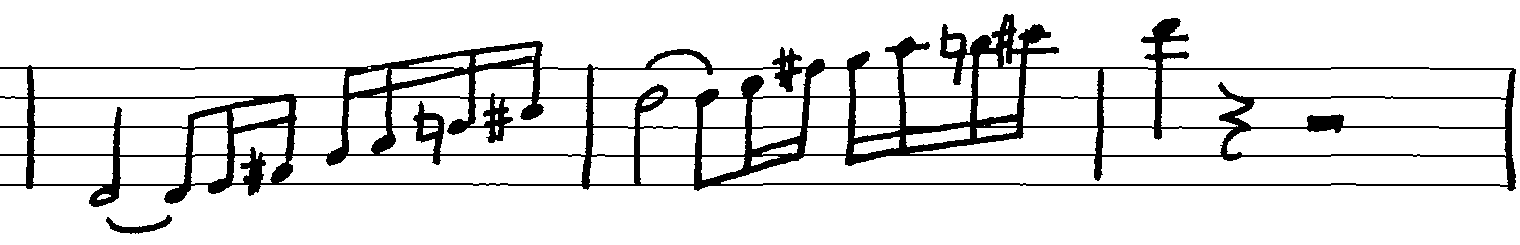
\includegraphics[width=130mm]{../img/comparison-real}
    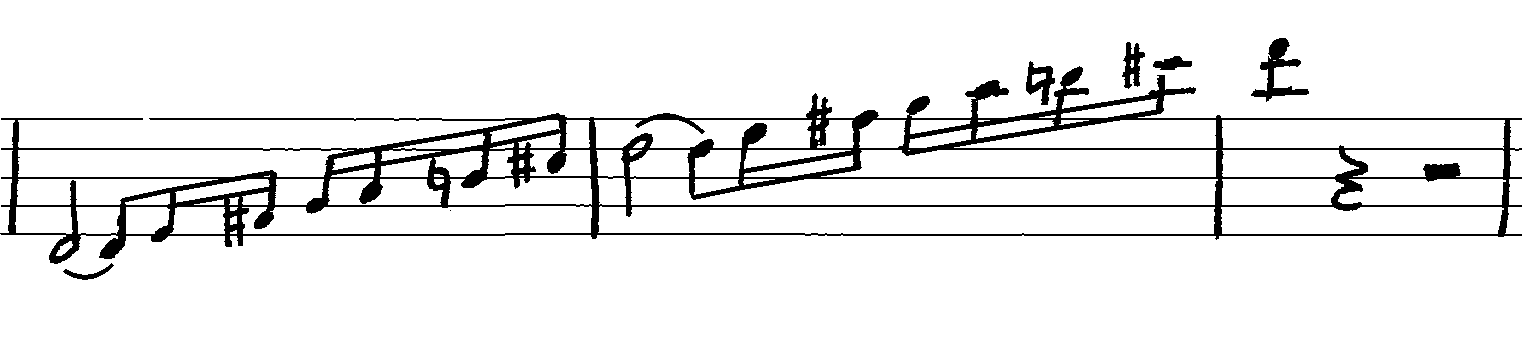
\includegraphics[width=140mm]{../img/comparison-engraved}
    \caption{
    Comparison of a real-world image to an engraved image. The top image is taken from the CVC-MUSCIMA dataset. The bottom image is the same music engraved using our engraving system and using symbols of the same writer.
    }
    \label{fig1:Comparison}
\end{figure}

It is difficult to evaluate an~OMR~system in general. This is because there is no standard dataset that can be used and no standard set of metrics. Moreover, we proposed a~new Mashcima representation for the music engraved in a~staff. This representation is based on the~agnostic encoding proposed by Calvo-Zaragoza and Rizo (\cite{Primus}). Using custom representation makes it yet more difficult to compare our results to other works. That being said, we can still make some comparisons. It seems that having a~specialized engraving system is a~step in the right direction. The results we obtained when evaluating are comparable to similar works performing similar evaluation (\cite{HmrBaseline}).

The~thesis assignment states that the~output of our model will be a~MusicXML file. We quickly realized that the~problem is far larger than anticipated and so we focused on the~core features only. Similarly, the~model input is not a~plain photo or scan. It is already preprocessed and binarized. This problem has already been solved during the~creation of the~CVC-MUSCIMA dataset (\cite{CvcMuscima}), therefore we didn't tackle it either.

Also, there's a~Github repository containing all the~source code and text of this thesis at \href{https://github.com/Jirka-Mayer/BachelorThesis}{\texttt{https://github.com/Jirka-Mayer/BachelorThesis}}. There's also a~release tag corresponding to the~time this thesis was submitted and it contains all the~trained models for download.

\section{Thesis Outline}

\paragraph{Chapter \ref{chap:Introduction}:} TODO

\paragraph{Chapter \ref{chap:RelatedWork}:} TODO

\paragraph{Chapter \ref{chap:DeepNeuralNetwork}:} This chapter describes the specific model we decide to use for our OMR task. It discusses traditional methods and how deep neural networks help us simplify the process. It describes models other people used for similar tasks and how we've been influenced by them.

\paragraph{Chapter \ref{chap:MusicRepresentation}:} This chapter mainly describes the Mashcima music encoding - the encoding we used for our model. It describes how it relates to the PrIMuS agnostic encoding, and why we made certain decisions regarding its design.

\paragraph{Chapter \ref{chap:EngravingSystem}:} This chapter talks about the Mashcima engraving system. Why we developed this system and what problem it solves. How it works, what are its limitations, and how it can be extended.

\paragraph{Chapter \ref{chap:ExperimentsAndResults}:} This chapter describes the experiments we performed. These experiments aim to measure the performance of our approach and test hypotheses postulated in previous chapters. We will also attempt to compare our results to other similar works.

\paragraph{Chapter \ref{chap:ConclusionAndFutureWork}:} TODO

\chapter{Related Work}
\label{chap:RelatedWork}


\section{CVC-MUSCIMA Dataset}
\label{sec:CvcMuscima}

CVC-MUSCIMA is a~dataset presented in the article: \emph{CVC-MUSCIMA: A ground truth of handwritten music score images for writer identification and staff removal} (\cite{CvcMuscima}). This dataset contains 1000~sheets of~music, consisting of 20~pages, each written by 50~different musicians. It is the~only publicly available dataset containing entire staves of handwritten music. The~dataset has been designed for writer identification and staff (staff line) removal tasks. It contains two sets of images. One set for writer identification (containing gray, binary, and staff-less binary images) and one set for staff removal (contains raw, staff-less, and staff-only images, all binary).

\begin{figure}[h]
    \centering
    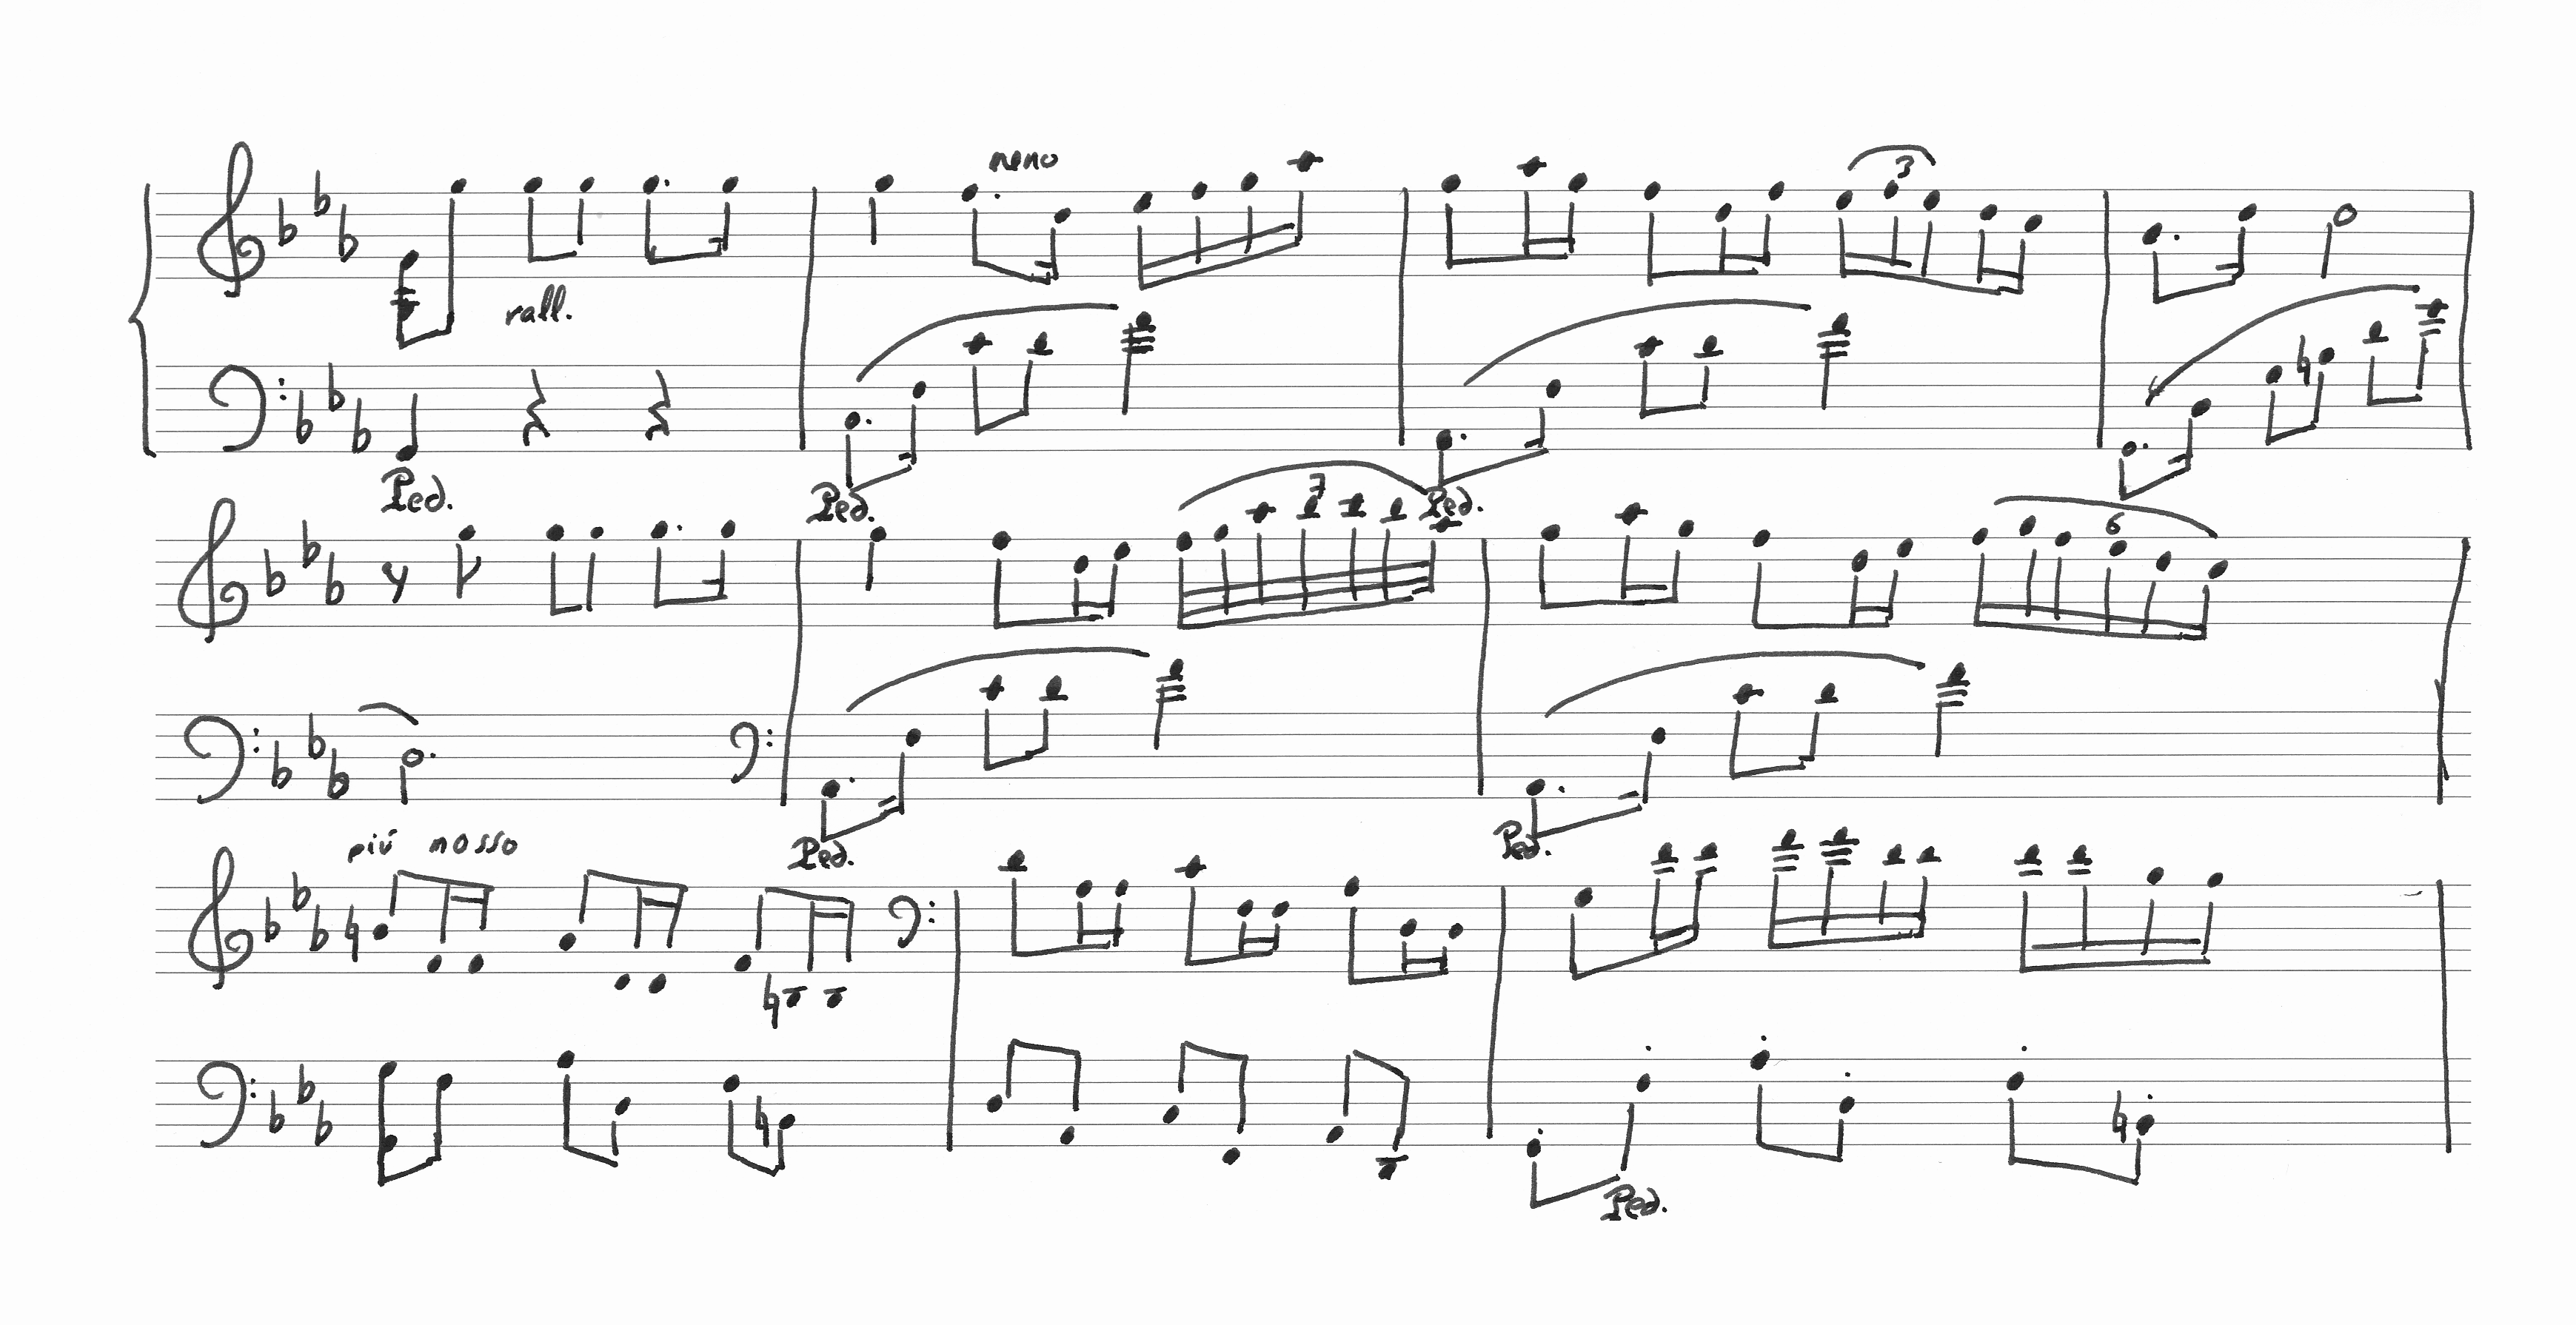
\includegraphics[width=140mm]{../img/cvc-muscima}
    \caption{One sheet of music from the CVC-MUSCIMA dataset. Image taken from the CVC-MUSCIMA website \href{http://www.cvc.uab.es/cvcmuscima/index_database.html}{\texttt{http://www.cvc.uab.es/{\allowbreak}cvc{\allowbreak}muscima/{\allowbreak}index\_database.html}}.}
    \label{fig2:CvcMuscima}
\end{figure}

We will use part of the~staff removal set for evaluation. We will also use another part of the~staff removal set for engraving, but indirectly via the MUSCIMA++ dataset.


\section{MUSCIMA++ Dataset}

MUSCIMA++ is a~dataset developed by Jan Hajič~jr. and Pavel Pecina and has been presented in the~article: \emph{In Search of a Dataset for Handwritten Optical Music Recognition: Introducing MUSCIMA++} (\cite{MuscimaPP}). This dataset provides additional information for a~subset of the~CVC-MUSCIMA dataset. MUSCIMA++ contains 140~sheets of music. Each sheet is annotated at the~level of individual symbols (noteheads, stems, flags, beams, slurs, staff lines). Each one of these symbols is classified, contains a~bounding box and a~pixel mask. These symbols are then interlinked in a~graph that can be traversed to extract higher-level objects (notes, key signatures, beamed note groups).

\begin{figure}[h]
    \centering
    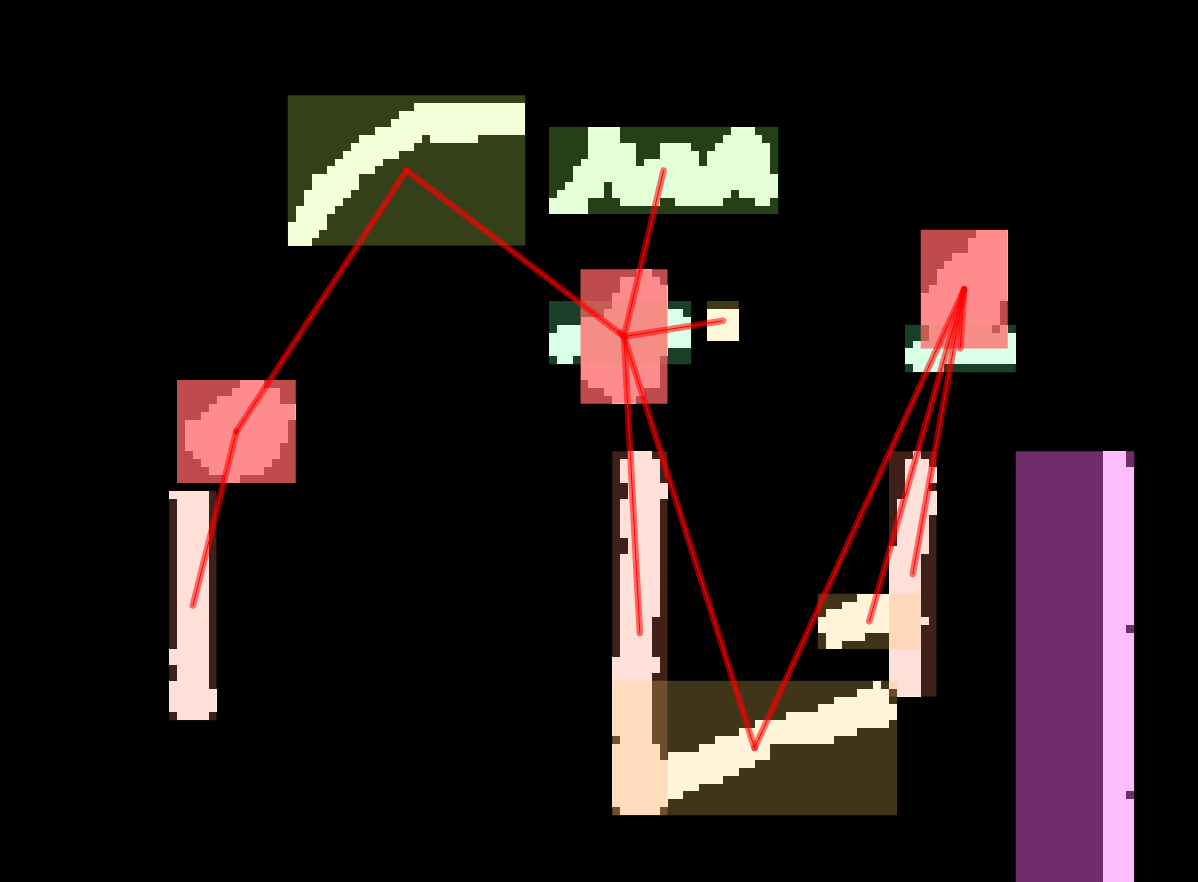
\includegraphics[width=100mm]{../img/muscima-pp}
    \caption{Notation graph of the MUSCIMA++ dataset. Image taken from \cite{MuscimaPP}.}
    \label{fig2:MuscimaPP}
\end{figure}

We will use the~dataset as a~collection of musical symbols. We will then place those symbols onto an~empty staff to create synthetic training data. The additional data (relationship graph) will help us position certain symbols properly.


\section{End-to-End OMR and the PrIMuS Dataset}

This section refers to the~article: \emph{End-to-End Neural Optical Music Recognition of Monophonic Scores} (\cite{Primus}). This article first describes the~PrIMuS\footnote{\href{https://grfia.dlsi.ua.es/primus/}{https://grfia.dlsi.ua.es/primus/}} dataset. This dataset contains 87678~real-music incipits. An~incipit is the~part of a~melody or a~musical work that is most recognizable for that work. Each incipit is a~few measures long, typically shorter than a~single staff of printed sheet music. Each incipit is encoded in a~few widely known encodings (MEI, MIDI) and has a corresponding printed image. This image has been engraved using the~music notation engraving library Verovio\footnote{\href{https://www.verovio.org/}{https://www.verovio.org/}}. Each incipit is also encoded using two on-purpose devised encodings --- the PrIMuS semantic and agnostic encoding. These encodings are interesting because they are the~output of a~model proposed in the~article, but also the~Mashcima encoding described in chapter \ref{chap:MusicRepresentation} of this thesis is very similar to the~agnostic encoding.

\begin{figure}[h]
    \centering
    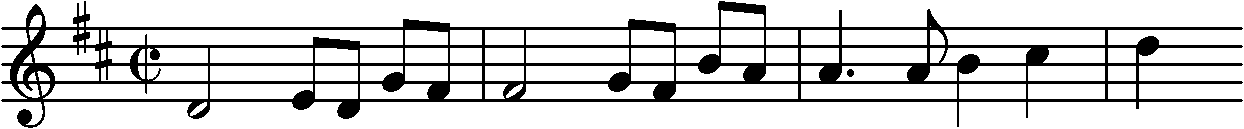
\includegraphics[width=120mm]{../img/primus-incipit}
    \\
    \medskip
    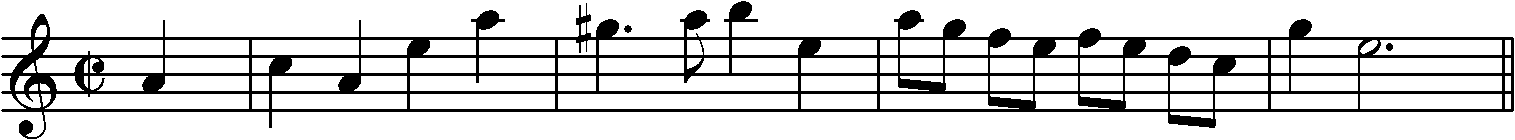
\includegraphics[width=140mm]{../img/primus-incipit-2}
    \caption{Two incipits taken directly from the PrIMuS dataset.}
    \label{fig2:PrimusIncipits}
\end{figure}

The~article also proposes a~neural network architecture for an~end-to-end solution of~OMR. The~architecture is very similar to ours, almost identical. It also uses the~connectionist temporal classification as the loss function (\cite{CTC}), which shapes the~PrIMuS dataset encoding formats. This thesis differs from this article mainly in the~focus on~handwritten music and the~introduction of~a~custom engraving system for handwritten music. The PrIMuS article focuses on~printed music only.

We will use the~PrIMuS dataset as a~source of~melodies that can be used as~input to~our engraving system. We will also take this article as~a~basis for our Mashcima encoding and our model architecture.


\section{HMR Baseline Article}

This section refers to the~article: \emph{From Optical Music Recognition to Handwritten Music Recognition: A baseline} (\cite{HmrBaseline}). This paper proposes a~model that should serve as a~baseline for handwritten music recognition. The model is again a~convolutional recurrent neural network that recognizes entire staves. The model is trained on~printed music and then, using transfer learning, fine-tuned on handwritten music. The handwritten music comes from the~MUSCIMA++ dataset and it has been varied using data augmentation (blurring, erosion, dilation, measure shuffling). This model, however, does not use the CTC loss function, instead, it produces two vectors for each pixel of the~input image width. One vector contains symbols that are present in the~image at~that position and the~other vector contains pitches of~these symbols. This means annotations have to be aligned with the symbols (unlike with CTC), but it allows the~model to recognize dense music sheets and even chords.

We will attempt to compare our model to the~one from this article. The~comparison will be difficult because the~output formats are so~different, but we will mention all the~differences and add a~qualitative comparison of the~final predictions. We want to utilize the fact that our evaluation dataset intersects with theirs and~so we can perform a~direct comparison.

\chapter{Deep Neural Networks}
\label{chap:DeepNeuralNetwork}

This chapter talks mainly about the~model we decided to use. First, we describe the~full pipeline of a~traditional OMR system. Many of these steps are shared between traditional and deep learning approaches. Then we will talk about the~deep learning approaches that can be taken. Neural networks can replace parts of a~traditional pipeline, or they can be used in an~end-to-end setting, where the~neural network replaces the~most difficult core of the~pipeline. We will describe our architecture consisting of a~convolutional block, recurrent block, and the~connectionist temporal classification (CTC) loss function. The~following sections describe in more detail what a~neural network is and how the~individual blocks of our model work internally. The~last section explains how CTC works and what are its pros and cons, compared to the~approach described in the~HMR baseline article (\cite{HmrBaseline}).


\section{Traditional Approaches}

A~musical score intended for OMR typically begins as a~raster image. This image is a~photo or a~scan of a~real-world sheet of paper. The~image needs to be prepared first. We need to find the~sheet of paper in the~image and correct any rotation or~perspective distortion. Scanned images are easier to~prepare because they do not contain any perspective deformation and lighting artifacts. Searching for the~paper in the~image can be performed using many approaches, e.g. by using maximally stable extremal regions (\cite{MSER}). We can detect staff lines using Hough transform (\cite{Hough}). We can then use this information to remove any affine distortion of the~image.

The~next step is performing some color normalization and binarization. There might be a~light-intensity gradient over the~image, so we do some automatic contrasting to bring the~lightness to a~constant level across the~image. Median filtering can be applied to remove noise (\cite{MedianFiltering}). Conversion to a~grayscale image is often used since colors are not useful to OMR. The~image can then be binarized to further remove unnecessary information. Many thresholding algorithms can be used for this step, many of which are implemented in the~OpenCV\footnote{\href{https://opencv.org/}{https://opencv.org/}} library. Binarization is important for traditional approaches since they often use methods based on connected components to detect individual symbols. Neural networks could benefit from non-binarized images since binarization can create aliasing artifacts that distort the~input image on the~pixel level.

The~steps described above are shared by both traditional and neural network-based approaches. Traditional approaches now usually perform staff line removal. This step lets methods based on~connected components to become useful. Staff localization may be an~important part of this step. Symbols then need to be segmented and classified separately. Meaning is then reconstructed by looking at the~relationships between all the~classified symbols. With the~musical score understood at the~symbol level, the~extracted information can be converted to some final representation (MusicXML, MEI, MIDI).


\section{Deep Learning Approaches}

Deep learning is a~class of machine learning that focuses on deep neural networks. Deep learning has risen over the~past two decades and became a~very powerful tool for solving many problems, especially classification problems regarding computer vision. Neural networks can be used in many places throughout the~pipeline of a~traditional OMR system. They can be used for staff line removal (\cite{CalvoZaragoza2017}), symbol classification (\cite{Lee2016}), or even symbol detection (\cite{Pacha2018}).

Recently, neural networks have been used to tackle the~problem of~OMR in an~end-to-end fashion (\cite{Primus}, \cite{HmrBaseline}). This approach allows us to replace many stages of the~pipeline with a~single model. The input sheet of music is usually processed staff by staff, so an~initial segmentation of staves is required. This step is, however, very robust and can be performed reliably.

The~main steps unified by an~end-to-end system are segmentation, symbol classification, and part of the~relationship extraction. This means we do not need to explicitly specify the~structure of this part of the~pipeline, which saves a~lot of time and thinking. Also, any intermediate features that would be extracted (like noteheads) need not be specified. The deep neural network can learn, what those features are. Moreover, it can adapt these features to the problem better than a~human could.

Deep learning, especially in an~end-to-end approach also has some drawbacks. The first is bound to the ability of the~model to learn the~solution from data. While it is very helpful, that we do not have to design part of our OMR system manually, it is often very difficult to acquire enough high-quality data for the~training. Also, the~more complex our model is and the~more learned parameters it has, the~more training data it requires. The~data also needs to be of high quality. Ambiguity and mistakes in annotations lead to poor performance of the~resulting model. The~trained model can only ever be as good as its training data.

The second drawback is the~very difficult nature of debugging the~model. A neural network is by design a~black box and we cannot easily assign specific meaning to any of its internal parts. The process of fixing a~mistake the model makes is tedious and requires a~lot of experimentation and re-training.


\section{Our Architecture}

As stated in the~title of this thesis, we decided to explore the~end-to-end approach to OMR using deep neural networks. We were primarily inspired by these three models:

\begin{itemize}
\item End-to-End Neural Optical Music Recognition of Monophonic Scores by Calvo-Zaragoza and Rizo (\cite{Primus})
\item SimpleHTR by Harald Scheidl\footnote{\href{https://github.com/githubharald/SimpleHTR}{https://github.com/githubharald/SimpleHTR}}
\item From Optical Music Recognition to Handwritten Music Recognition: A baseline (\cite{HmrBaseline})
\end{itemize}

All of these models share the~same high-level structure. They combine a~convolutional neural network (CNN) with a~recurrent neural network (RNN). This combination is sometimes called RCNN architecture. Convolutional neural networks are used in image processing. Their architecture is inspired by the~way filters work in computer graphics (convolving a~kernel over the~source image). They learn to extract edges, corners, and then even more abstract features like noteheads and stems. Recurrent neural networks are used for sequence processing (text and speech). They have been designed to carry state information throughout the~input sequence. In our case, they learn to propagate information horizontally - like inferring pitch of an~accidental from the~pitch of a~neighboring note. The CNN block learns to extract features that the RNN block then learns to combine into more abstract features.

\begin{figure}[h]
    \centering
    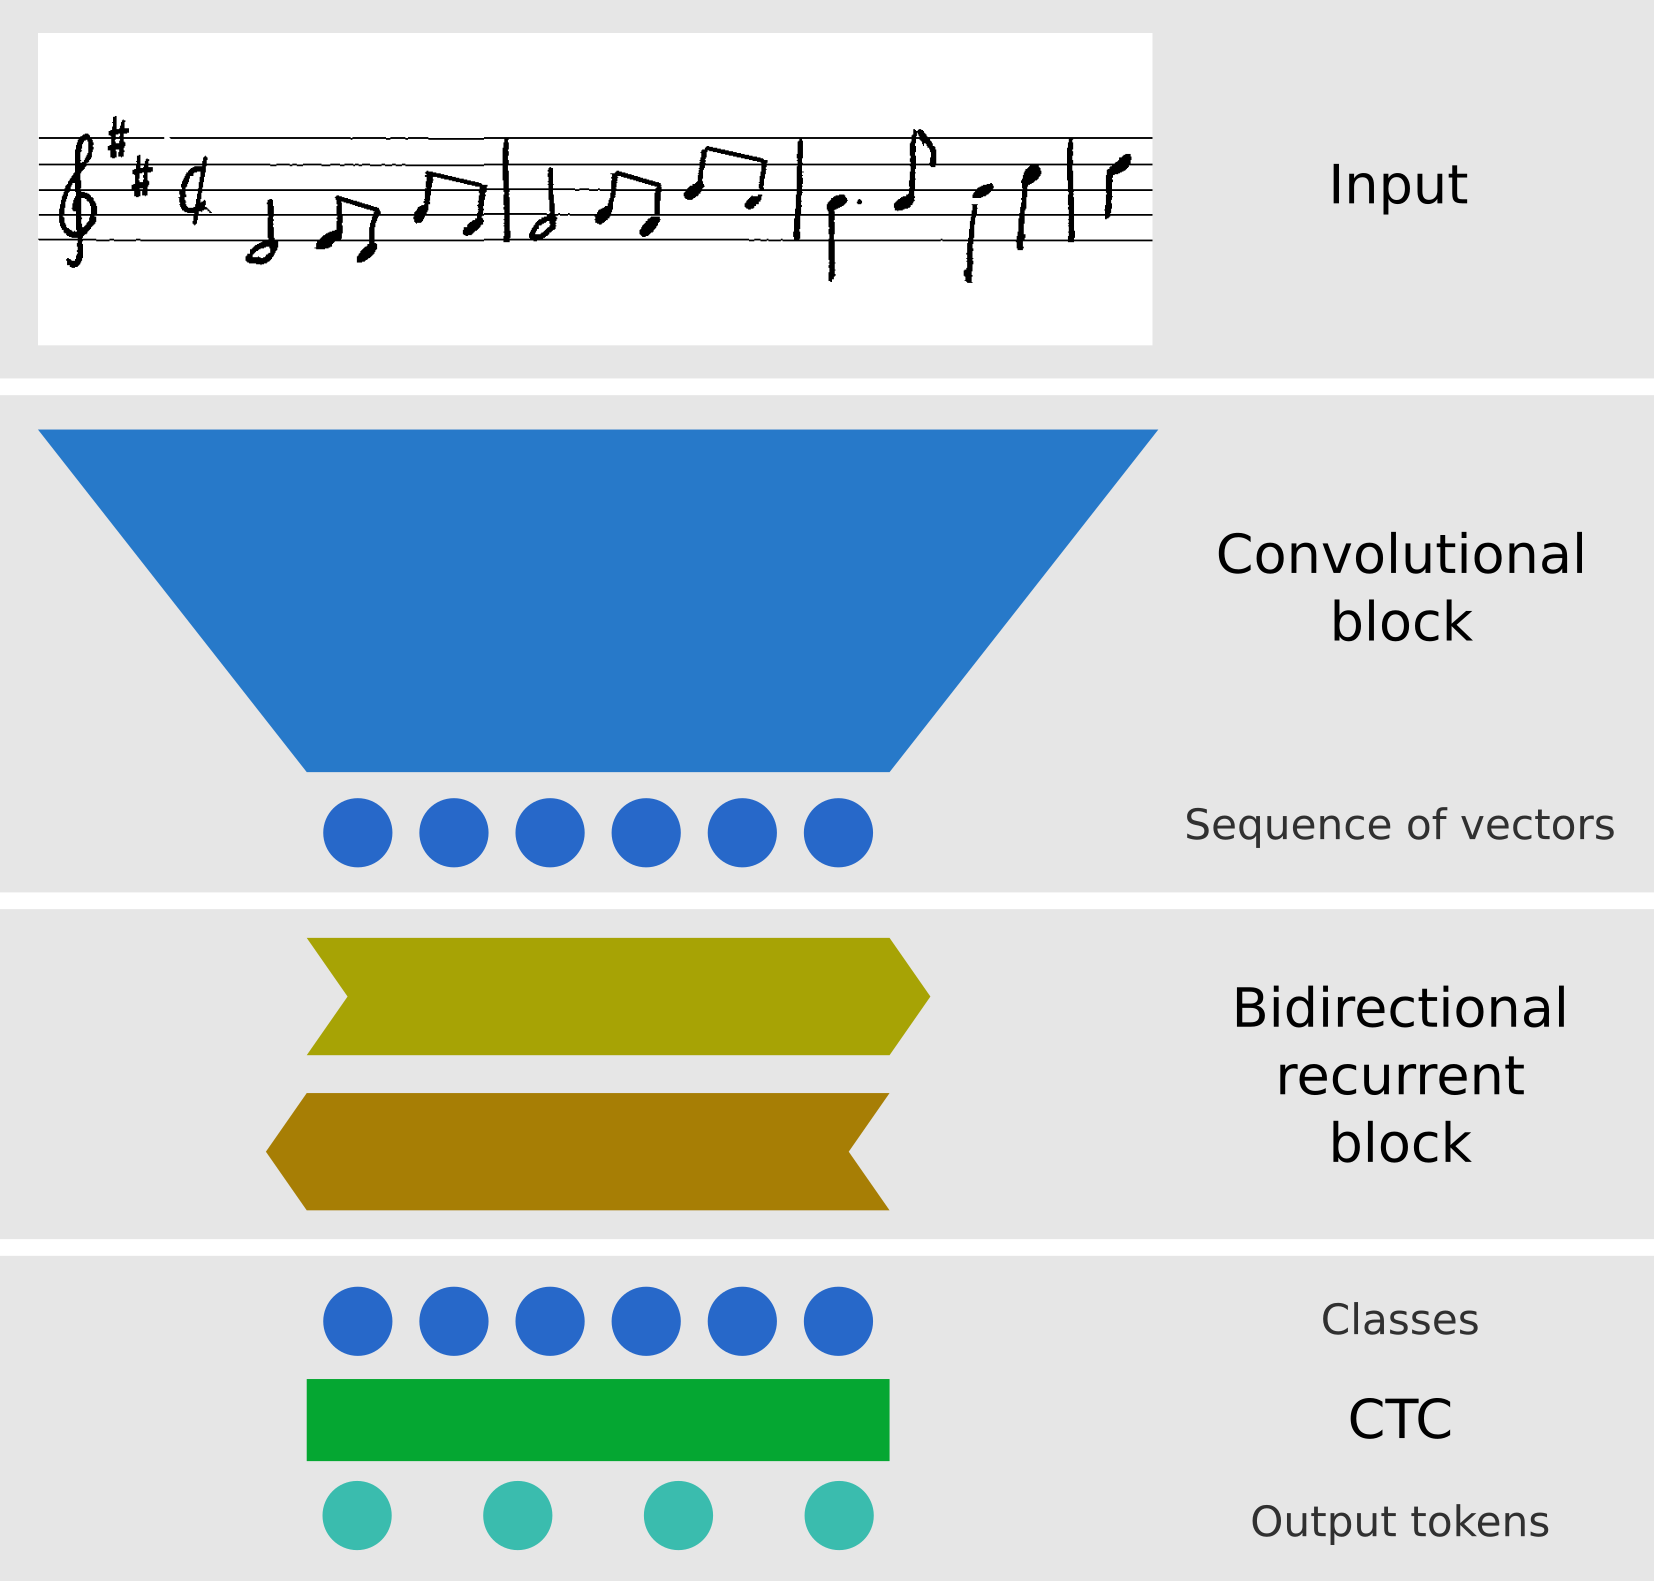
\includegraphics[width=140mm]{../img/network-architecture}
    \caption{Diagram of our model --- a RCNN network with CTC loss function. Detailed list of layers with all parameters can be found in table~\ref{tab6:NetworkLayers}}
    \label{fig3:NetworkArchitecture}
\end{figure}

The~CNN block can be followed by fully connected layers that further refine the~result, although these layers are not necessary and our architecture does not contain them. This may be due to the fact that our encoding is very close to the~symbolic visual representation and~so most of the~heavy lifting is probably performed in the~CNN block.

The~final layer outputs a~sequence of vectors, where each vector represents one time-step (horizontal slice of the~input image). Values in such vector correspond to probabilities of individual output classes (tokens) at that given time-step. One additional class \emph{blank} is added, which represents "no symbol present". The~most likely class for each time-step is selected and then repetitions of the~same class are collapsed into one token. Lastly, all the~blank symbols are removed. The~remaining sequence of classes is mapped directly onto annotation tokens of the~Mashcima encoding explained in the~chapter \ref{chap:MusicRepresentation}. This approach is called greedy CTC decoding (\cite{CTC}) and is used during training. For evaluation, a more advanced method is used, called beam search decoding (\cite{CtcBeamSearch}).

When training, the~loss is computed using the~connectionist temporal classification. The~loss function provides a~gradient for improving the~network. This gradient is then calculated for the~entire network using the~backpropagation algorithm (\cite{Goodfellow-et-al-2016}). Parameters are then updated using the~adaptive learning rate optimizer (Adam) (\cite{AdamOptimizer}).

The~values of all hyperparameters, including sizes and types of all layers, are specified in the~section \ref{sec:ArchitectureTrainingEvaluation}.


\section{Neural Network}

A~neural network is a~model inspired by the~human brain. Its~core building block is a~perceptron (analogous to a~neuron in the~brain). Perceptron is a~node that has several inputs (real numbers), combines them, and produces a~single output value. The mathematical description is the following:

$$
    y = \varphi(w \cdot x + b)
$$

Vector $x$ contains all the~input values. It is multiplied by a~vector of weights $w$ and a~constant scalar bias $b$ is added. The~result is passed through an~activation function $\varphi$ that produces the~output value $y$. The~core idea behind this model is that a~perceptron activates (fires) when enough inputs activate. Weights and the~bias are parameters that allow the~perceptron to learn - to detect a~specific pattern in the~input values. The~activation function attempts to model the~activation threshold and introduces non-linearity into the~system.

One of the~first activation functions to be used was the~sigmoid function, but~it suffered from the~problem of vanishing and exploding gradients (\cite{VanishingGradient}). The hyperbolic tangent function was then used to remedy this problem. Nowadays, rectifier function is often used ($\max(0, x)$), because it is easy to compute. Perceptrons with this function are called rectified linear units (ReLU). It~also has some problems, so~leaky ReLU can be used to address them (\cite{Maas2013RectifierNI}).

\begin{figure}[h]
    \centering
    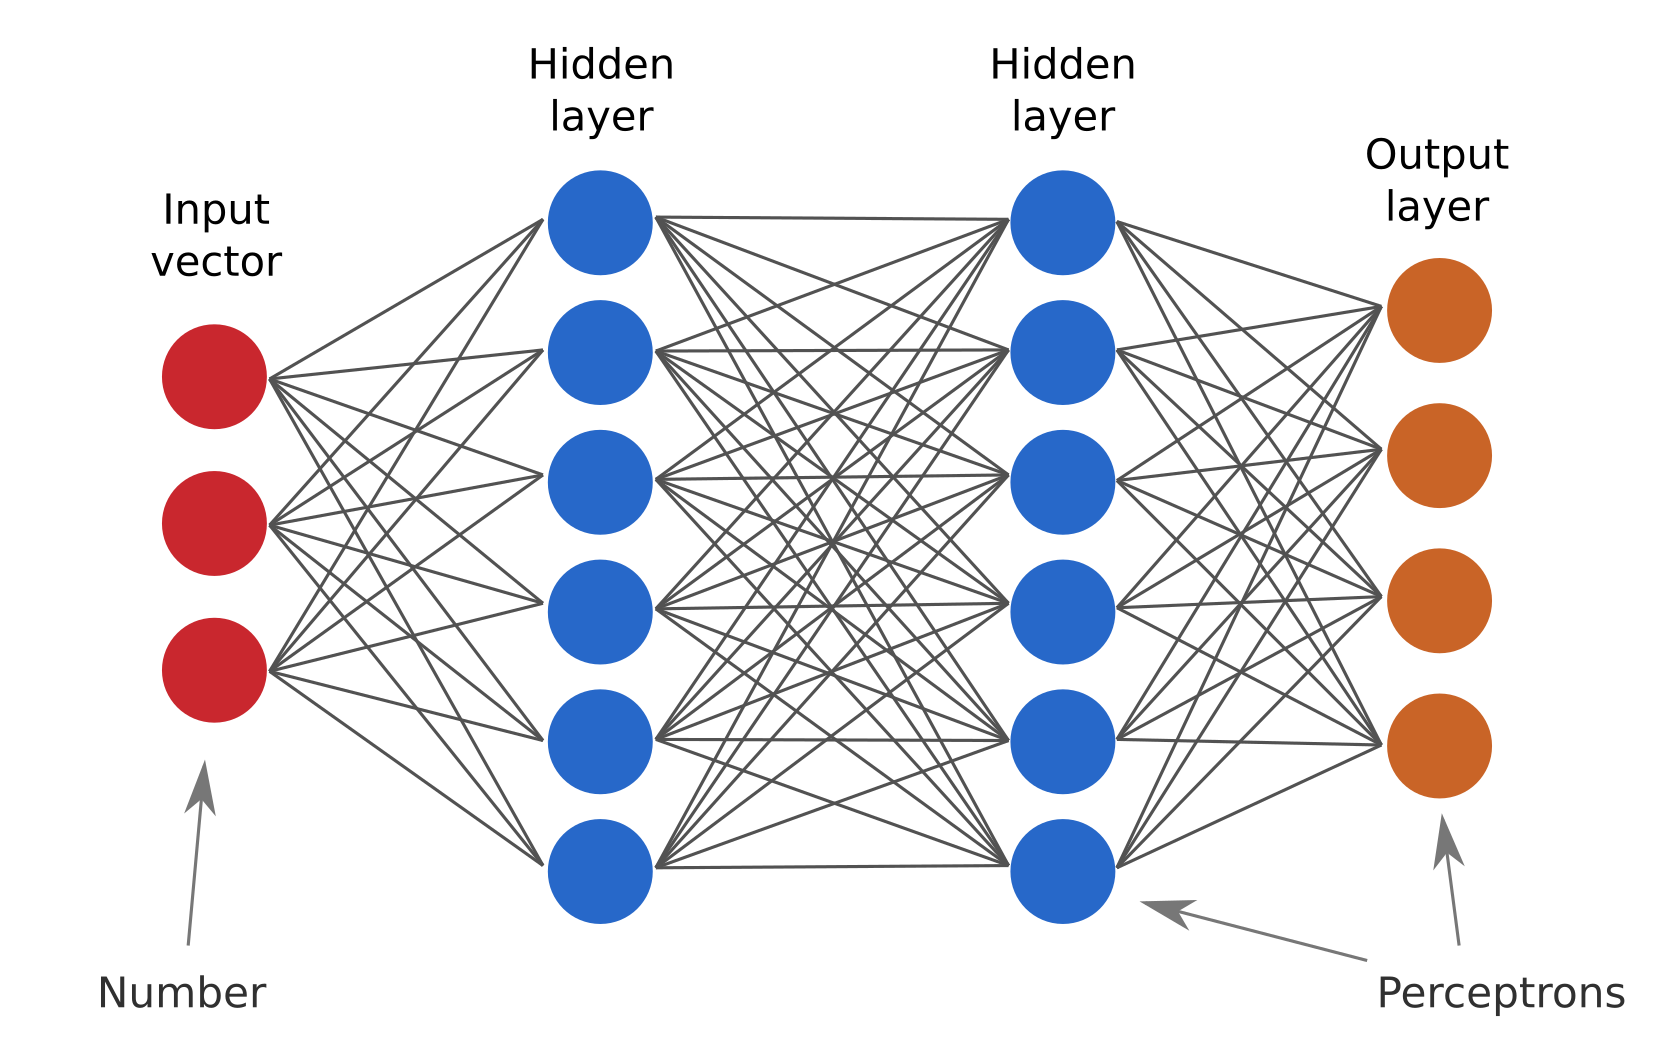
\includegraphics[width=140mm]{../img/neural-network}
    \caption{Fully-connected neural network with 3 layers.}
    \label{fig3:NeuralNetwork}
\end{figure}

Perceptrons can be interconnected to form neural networks. A~typical architecture is a~feedforward neural network (FNN). It~organizes perceptrons into layers, through which information flows in one direction. The resulting graph is directed and acyclic, which allows us to understand the~whole network as a~complex mathematical function and lets us train it using the~backpropagation and gradient descent algorithms (\cite{Goodfellow-et-al-2016}).

The~simplest feedforward network is a~network with dense (fully connected) layers. Each perceptron in a~given layer receives input as the~output of all perceptrons in the~previous layer.


\section{Convolutional Neural Network}

A~convolutional neural network (CNN) is a~kind of feedforward network. It~is ideal for processing visual data. A~CNN is built primarily from two kinds of layers:

\paragraph{Convolutional layer} A~convolutional layer is similar to a~fully connected layer, but the~connections are only local. The~input and output is a~two-dimensional array of numbers (like one channel of an~image). Each perceptron takes input from only a~small window of neighboring perceptrons in the~input layer (\texttt{3x3}, \texttt{5x5}, \texttt{7x7}). Weights are represented by a~kernel of the~same size as this neighborhood window. This kernel is shared by all the~perceptrons, reducing the~number of learned arguments substantially and allowing the~layer to process images of variable sizes. There may be multiple input and output arrays (channels). In such a~case, the~convolutional layer has one kernel for each pair of channels. This architecture is inspired by the~convolution filters from computer graphics --- hence the name.

\begin{figure}[h]
    \centering
    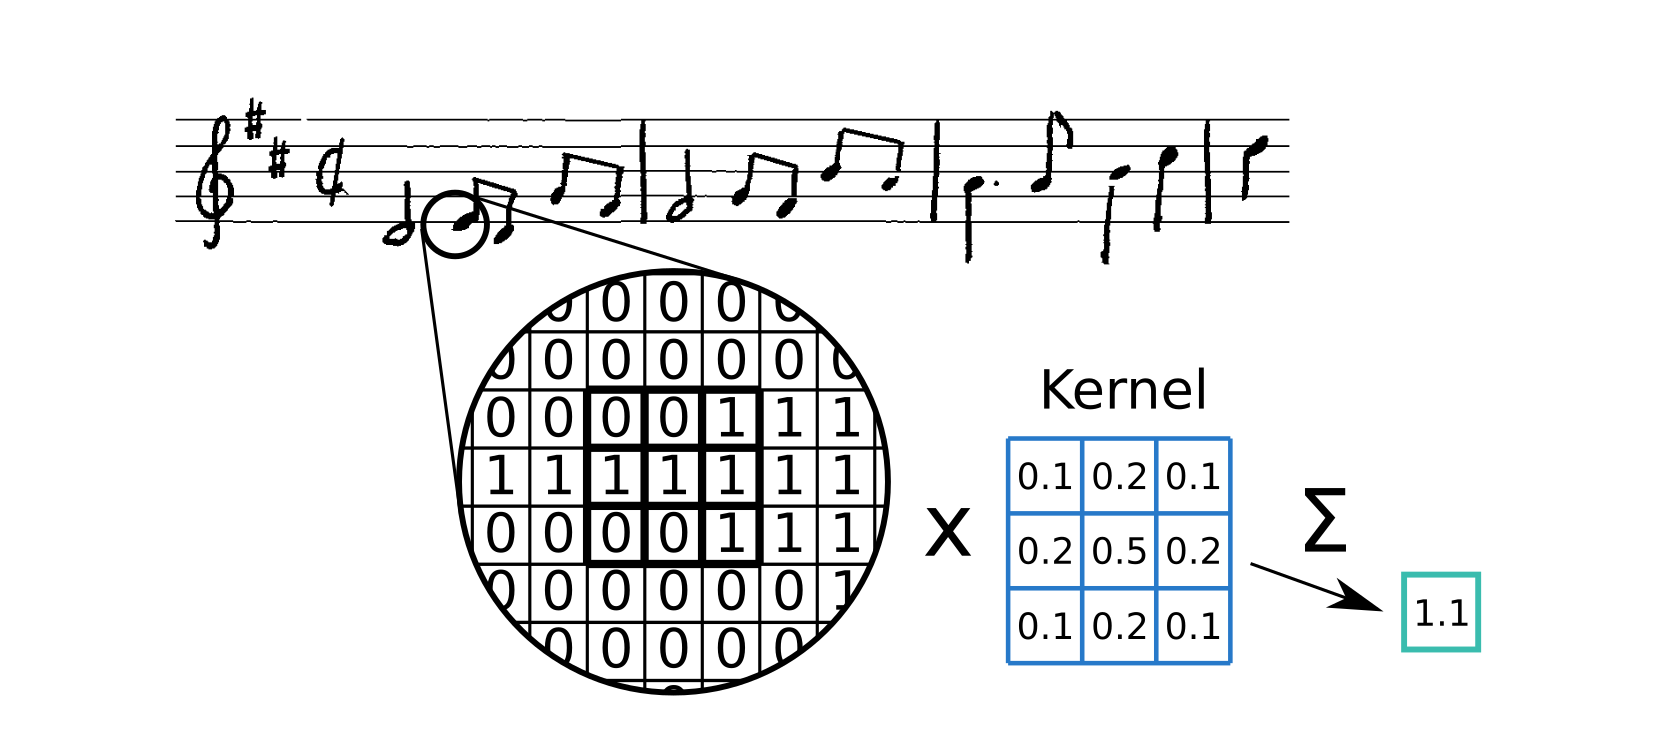
\includegraphics[width=140mm]{../img/convolution}
    \caption{Computation of one output pixel in a convolutional layer.}
    \label{fig3:Convolution}
\end{figure}

\paragraph{Pooling layer} A~pooling layer typically follows a~convolutional layer. Its~job is to downsample the~image, reducing its spatial resolution, while preserving the number of channels. The~downsampling is performed by splitting the~input into a~set of rectangular regions (that may overlap) and then reducing each region using max, sum, or average operator. Widely used is the~maximum operator and the~resulting layer is called a~\emph{max pooling layer}. The pool size is typically \texttt{2x2}.

\paragraph{Fully-connected layer} One or more fully connected layers can be added at the~end of a~CNN, to further refine features extracted by the~previous layers. This layer is often present in models performing classification because we want to reduce the~number of outputs to the~number of classes we are predicting.

A~CNN has typically many convolutional layers, combined with pooling layers. Each time the~spatial dimensions shrink in a~pooling layer, more channels are added to be able to represent more features. This forces the network to create abstractions and convert the~visual data into some abstract representation vector.


\section{Recurrent Neural Network}

A~recurrent neural network (RNN) is a~network intended for sequence processing. Input for the~network is a~sequence of vectors and the~output is a~sequence of the~same length. The~recurrent network can be understood as composed of recurrent units, each with two inputs and two outputs. A~unit accepts one vector from the~input sequence and an~old state vector. It~outputs the~corresponding vector of the~output sequence and the~new state vector. These recurrent units can be unrolled along the~input sequence and each one passes the~state vector to the next one, using it to send information along the~length of the~sequence. All instances of the~recurrent unit share the~same learned parameters and so can be unrolled to any length necessary. The~sequence dimension, where unrolling happens, is called the time dimension.

\begin{figure}[h]
    \centering
    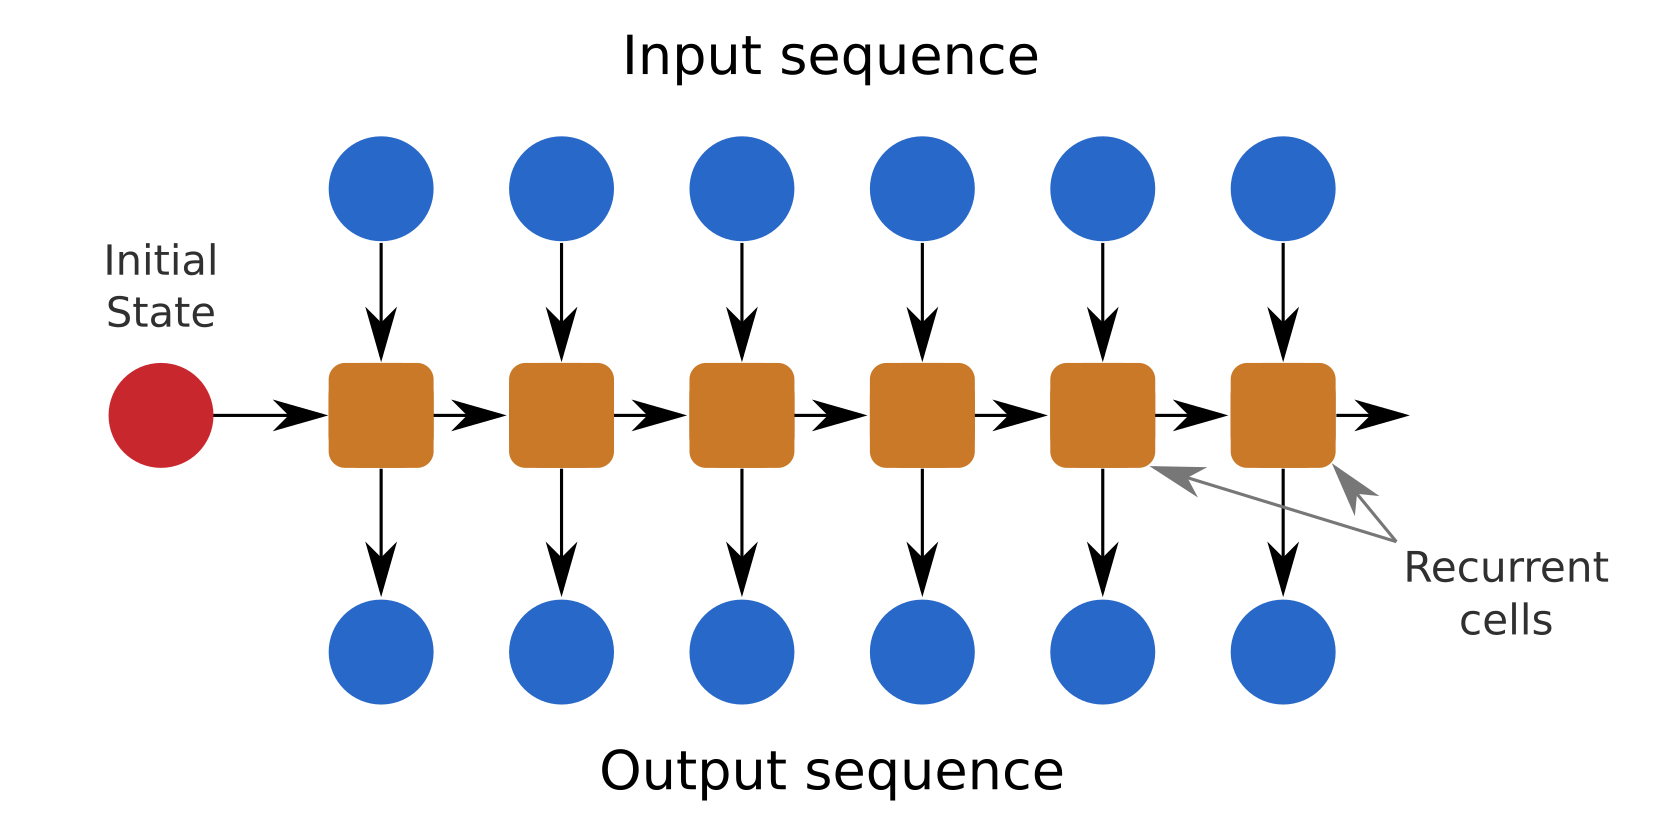
\includegraphics[width=140mm]{../img/recurrent-network}
    \caption{Unrolled recurrent units processing a sequence of vectors.}
    \label{fig3:RecurrentNetwork}
\end{figure}

The~internal architecture of a~recurrent unit may vary, but it is often a~feedforward network, where the~input and output vectors are both split into a~sequence part and a~state part. The most common recurrent unit architectures are the~long short-term memory (LSTM) (\cite{LSTM}) and the~gated recurrent unit (GRU) (\cite{GRU}). You can join two recurrent layers, passing information in opposite directions, to create a~bidirectional recurrent layer.


\section{Connectionist Temporal Classification}

A~recurrent neural network outputs a~sequence of vectors. If~these vectors are the~final output of the~model, they typically represent class probabilities for a~given time-step (we solve sequence classification). If~we did OCR, we~would have a~set of characters (an~alphabet) and the~vector would have the~same size as the~alphabet. Each value in that vector would correspond to the~probability of that given character being present at that given time-step. We could use the~softmax function (\cite{Goodfellow-et-al-2016}) to convert the perceptron activations to probabilities.

This creates a~problem when training. In~OCR, we want to produce a~sequence of letters as the~output. But one letter might span multiple time-steps in the~input. This means we not only need the~gold sequence of letters, but we also need to know at which specific time-steps the~letters are present. This mapping of output classes to specific time-steps is called \emph{alignment} and it complicates the~creation of a~training dataset.

Connectionist temporal classification (CTC) (\cite{CTC}) is an~approach that solves the~alignment issue. The CTC loss function can calculate the~loss value over all possible alignments of our gold sequence over the~output sequence. This allows us to train the~model, without having explicit alignment.

When the~model is trained, the~greedy decoding algorithm (\cite{CTC}) can be used to convert the~output vector sequence to the~proper prediction. This algorithm takes each vector of the~output sequence and selects the~most probable output class (letter). It~then collapses all repetitions of that class into one occurrence, producing the~final sequence. One special output class called \emph{blank} is introduced, to prevent two actual successive occurrences of a~given class from being collapsed into one. This symbol is, however, after collapsing removed and will never be present in the~final prediction.

There is also the~option to use the beam search decoding algorithm (\cite{CtcBeamSearch}). This algorithm keeps a~list of best decodings so~far, as the~entire decoding is being computed. Greedy decoding is a~special case of the~beam search decoding, where the~list contains only one item. All partial decodings cannot be considered, because there are exponentially many of them.

The~connectionist temporal classification has many benefits regarding the alignment problem, but it has some flaws as well. The~loss computation and the~decoding rely on the~fact, that there will be only one class predicted for each time-step. This means we cannot capture the~fact of two symbols appearing in the~input at the~same time. This happens often with music. We can solve this problem partially by utilizing the~recurrent layers. They will allow us to output simultaneous symbols sequentially, by remembering those symbols for a~while. This however increases the~length of the~final sequence, but this sequence can never be longer than the~total number of time-steps. We might run out of temporal resolution.

The~HMR baseline article (\cite{HmrBaseline}) opted not to use CTC and performed manual alignment instead. This lets them have a~model that can predict multiple symbols simultaneously. This also reduces the~complexity of the~output sequence and the~model thus need not perform much additional work as in our case (see the~section \ref{sec:Attachments} on attachment ordering).

\chapter{Music Representation}
\label{chap:MusicRepresentation}

\section{PrIMuS Agnostic Encoding}

\section{Mashcima Music Encoding}

\subsection{Notes And Pitches}

\subsection{Rests And Barlines}

\subsection{Generic Tokens}

\subsection{Attachments}

\subsection{Slurs}

\subsection{Beams}

\subsection{Key Signatures and Time Signatures}

\subsection{Clefs and Repeats}

\section{Differences to PrIMuS}

\section{Extensibility}

\chapter{Engraving System}
\label{chap:EngravingSystem}

This chapter describes the Mashcima engraving system we developed. We created a~custom engraving system for handwritten music to serve as an~advanced data augmentation tool. We opted to write a~new system from scratch, because of the flexibility we needed. We will talk about the specific requirements for the engraving system. We will briefly overview the inner workings of the system - how it understands the input (Mashcima encoding), what are the basic building blocks from which a~staff image is engraved, what are the most important events that happen during engraving. We will talk about the shortcomings of the system and how it could be extended in the future.


\section{Why Custom Engraving System}

In the thesis introduction (chapter \ref{chap:Introduction}) we stated that there is only a~single dataset containing handwritten staves of music. There are other handwritten music datasets, but they either contain only symbols, or they are derived from CVC-MUSCIMA. Using this dataset as-is for training is not plausible, because it contains far too few symbol combinations.

We are not the first to realize this issue. The HMR baseline article (\cite{HmrBaseline}) talks about using data augmentation and transfer learning to solve the lack of training data. They propose a~model to be trained on printed music, of which there is abundance. After that, the model is fine-tuned by training on the CVC-MUSCIMA dataset. The results they obtained are impressive, considering the method they used. To help with the process, they used data augmentation, like dilation, erosion, and blurring, and even measure shuffling.

We propose to use more sophisticated data augmentation. Specifically, we want to shuffle the data on the level of individual musical symbols. The reason we choose this approach is that we have access to the MUSCIMA++ dataset (\cite{MuscimaPP}). This dataset contains a~lot of additional information regarding the CVC-MUSCIMA dataset, which includes segmentation masks of individual symbols and their relationships. We want to use these masks to engrave entirely new staves of music.

We will also build our own engraving system because engraving handwritten music is something that existing engraving systems do not focus on. Handwritten music is very different from printed music. Symbol positions vary, notehead shapes may differ from note to note within a~single staff, slant angle may also change. We tried looking at Abjad\footnote{\href{https://github.com/Abjad/abjad}{https://github.com/Abjad/abjad}} --- a~python package for engraving music that uses Lilypond\footnote{\href{http://lilypond.org/}{http://lilypond.org/}} at its core. Lilypond can load custom fonts, but those have to be in vector form, not raster masks. Also, there is no way to introduce a~controlled variability and randomness into the engraving process. When we considered the options, we decided to create or own system, since it would be faster and we would have the ability to modify it in the future.


\section{Requirements}

We are not trying to produce PDF files as the other engraving systems do. Our goal is to produce a~single staff of handwritten music, as a~raster image. This image should look as similar as possible to a~cropped image of a~staff from the CVC-MUSCIMA dataset. This means the image is already binarized, it has comparable resolution and the image has about three times the height of the staff it contains (the height of the staff lines).

This similarity can be accomplished by using symbols from MUSCIMA++. On page 19 of writer 1, there is an~empty staff. We take the mask of the staff lines and produce an~empty image of proper dimensions containing the empty staff lines. The staff lines are almost perfectly horizontal (they wobble up and down by a~few pixels, but do not drift), therefore we will use them to create a~lookup table for converting pitch numbers to pixel offset in the $y$ axis. This will act as our blank canvas, from which we will start. \emph{Canvas} is an~actual term used in the codebase.

\begin{figure}[h]
    \centering
    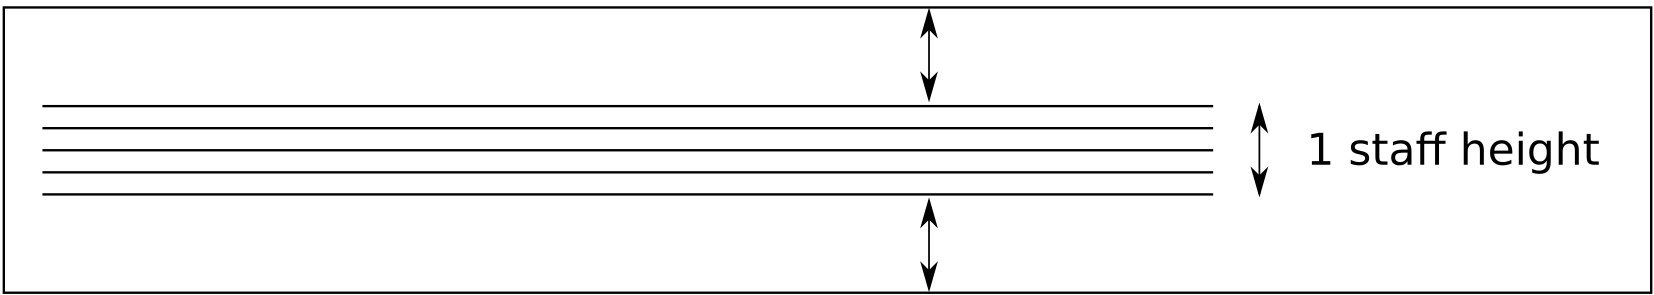
\includegraphics[width=140mm]{../img/staff-padding}
    \caption{Empty staff and the padding to the edge of the engraved image.}
    \label{fig5:EmptyStaffWithPadding}
\end{figure}

By trying to mimic the look of CVC-MUSCIMA, we will remove a~lot of problems that we would otherwise face. We do not need to perform any distortion removal, alignment, cropping, preprocessing, and binarization. All this is already performed on the source data we use. This lets us focus only on the engraving system, which is complicated enough by itself.


\section{Token Groups and Canvas Items}

The Mashcima encoding defines the concept of token groups. It is not discussed in the chapter on the encoding, because it is not so important for the encoding itself. A~\emph{token group} is a~group of tokens, that has one main token and then all the attachments of that token. So for example a~quarter note with a~sharp and a~staccato dot is represented by three tokens, but it is a~single token group. A~token group is all the tokens that belong to some non-attachment token.

Token groups are used in Mashcima annotation validation. When proper attachment ordering is checked, the annotation is first grouped into token groups and then each group has its attachment order checked. It also helps us to hide away all the attachment tokens and focus only on the important tokens.

Two special kinds of token groups are key signatures and numeric time signatures. It again makes sense to treat a~time signature as a~single object and since it is a~multitude of tokens, it is represented by a~token group.

Token groups are important because they map directly onto canvas items. A~\emph{canvas item} is something on the staff, that takes up horizontal space and can be rendered. Canvas item represents a~barline, a~note, a~rest. Attachments, like accidentals and dots, are not canvas items but are part of some given canvas item and they modify its appearance. Canvas items are placed on the staff right after each other with some randomized amount of padding between them. A~canvas item has all the vertical space it can have and it decides, where to draw itself vertically. You can see the bounding boxes of individual canvas items in figure~\ref{fig5:CanvasItems}.

\begin{figure}[h]
    \centering
    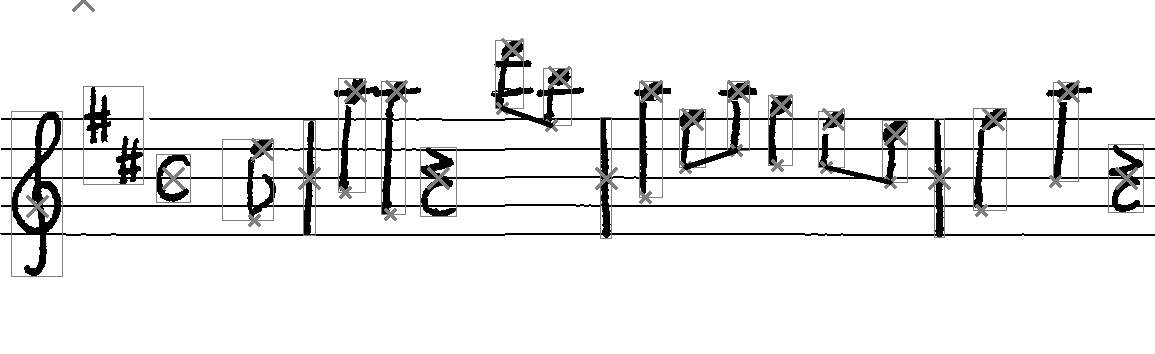
\includegraphics[width=140mm]{../img/canvas-items}
    \caption{Canvas items with bounding boxes. A bounding box encloses all sprites of a canvas item. The large cross is the origin and it used to position the items vertically. Smaller crosses are marking where a stem ends and a beam attaches. A key signature does not use its origin point, so it is left at the top of the image.}
    \label{fig5:CanvasItems}
\end{figure}


\section{Rendering Flow}

The process of converting an~annotation to an~image has a~couple of important steps:

\paragraph{Canvas instance is created} An~instance of the \verb`mashcima.`\allowbreak\verb`Canvas` class is created, so that canvas items could be added into it.

\paragraph{Canvas items are added} The annotation is grouped into token groups and those groups are mapped onto canvas items. This step just feeds the semantic information from the encoding system to the engraving system. This step is performed by the \verb`annotation_`\allowbreak\verb`to_canvas` function inside \verb`mashcima/`\allowbreak\verb`annotation_`\allowbreak\verb`to_image.py`.
\\

The following steps happen inside the \verb`Canvas`\allowbreak\verb`.render(...)` method.

\paragraph{Canvas construction is finished} This goes over the added canvas items and extracts information about slurs and beams. This step also validates that beams and slurs are properly formed. This extracted information is used later during the rendering of slurs and beams.

\paragraph{Sprites are selected} Each canvas item gets to choose specific symbol sprites (images) to use for rendering. These sprites are chosen from a~symbol sprite repository, represented by the class \verb`mashcima`\allowbreak\verb`.Mashcima` inside the file \verb`mashcima/`\allowbreak\verb`__init__.py`.

\paragraph{Sprites and canvas items are placed} With specific sprites selected, dimensions are now known and so everything can be positioned properly. Canvas items are positioned from left to right one at a~time. Each time a~canvas item is placed, it also places its internal sprites (and attachments and other ornaments) and determines its total width.

\paragraph{Beams are placed} With note positions known, we can calculate the proper position and angle for each beam. Once the beam position is calculated, the length of stems of all corresponding notes is adjusted to match the beam.

\paragraph{Everything is rendered} Canvas items, beams, and slurs are rendered. The order is not important, because the resulting image is binary.


\section{Slurs and Beams}

There are only a~few symbols that are not taken from the MUSCIMA++ dataset as images but are instead rendered manually. Those are slurs and beams. MUSCIMA++ does contain binary masks of these symbols, but the problem is that they cannot be simply moved to a~different position and rendered. They rely heavily on the position of other symbols and therefore they would need to be stretched, rotated, and skewed to render properly.

Slurs have some pre-defined attachment points they can use and the specific attachment point is chosen by the way a~note is flipped. Once the two points are chosen, the slur is rendered as a~parabola. This approach far too naive and simplified, so it does not capture the whole variability of a~handwritten slur. We think this is the reason the model makes so many mistakes regarding slur placement.

\begin{figure}[h]
    \centering
    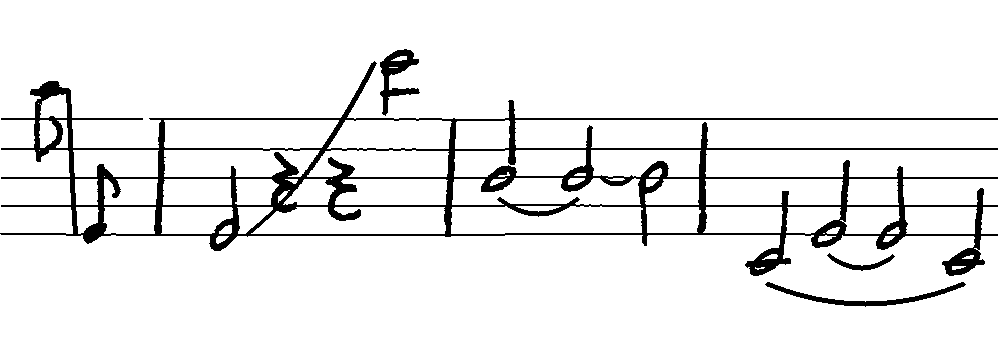
\includegraphics[width=120mm]{../img/failed-slurs}
    \verb`e6 ( ) e-4 | h-4 ( qr qr ) h8 | h0 ( ) h0 ( ) h0 |`
    \verb`h-6 ( h-4 ( ) h-4 ) h-6`
    \caption{Sometimes slur rendering does not look nice. Slurs cannot move other items around or create additional space. Slur does not move away when it intersects other symbols. Nested slurs are allowed, although not recommended.}
    \label{fig5:FailedSlurs}
\end{figure}

Beams face many similar problems as slurs. They are also rendered manually, as straight lines. This again does not capture the real world. Beams are often curved or they have a~gap between themselves and note stems. This again seems to be the source of many mistakes, especially with the writer 49, who leaves a~lot of gaps between beams and stems.


\section{Multi-staff images}

Staves are usually so close together, that cropping a~single staff with proper space around it will usually crop parts of symbols from the staves above and below. We want to capture this property of real-world data in our synthetic data.

We can take our rendering system and run it three times to render three staves into a~single image. We crop out the middle staff we actually want. It can be used with some variations --- having staff only above, or only below.

Multi-staff rendering can be performed by the \verb`multi_`\allowbreak\verb`staff_`\allowbreak\verb`annotation_`\allowbreak\verb`to_image` function inside \verb`mashcima/`\allowbreak\verb`annotation_`\allowbreak\verb`to_image.py` file.

\begin{figure}[h]
    \centering
    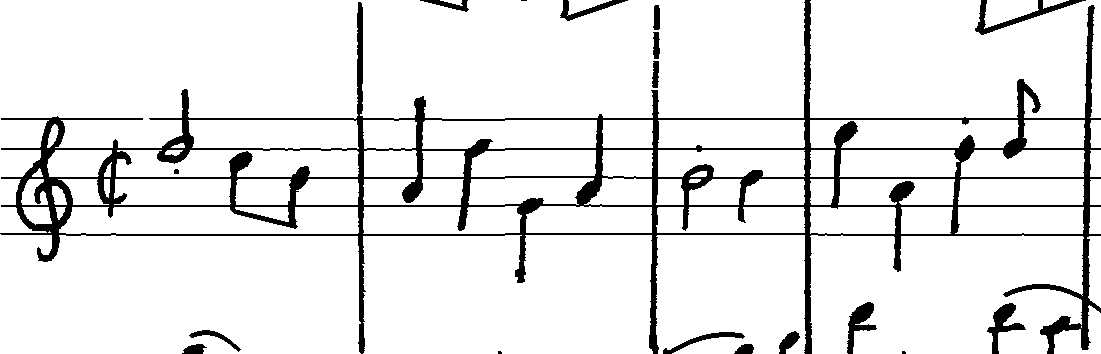
\includegraphics[width=120mm]{../img/multi-staff}
    \caption{Rendering staves above and below with long barlines.}
    \label{fig5:MultiStaff}
\end{figure}


\section{Additional Deformation and Normalization}

Affine transformation is applied to the produced image to make the model resilient to changes in image positioning, perspective, size, and rotation. This transformation is a~subtle, but very important step of the synthetic data preparation.

Finally, before the image is fed into the model, it is normalized to a~specified height, while preserving the aspect ratio. The resulting image can look like this:

\begin{figure}[h]
    \centering
    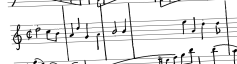
\includegraphics[width=120mm]{../img/normalized-image}
    \caption{Skewed and normalized to 64 pixels in height. The blurriness is not an artifact of engraving this thesis document, it is actually present in the data. The transformation and normalization turn the image grayscale, so the model takes grayscale images as input, not binary.}
    \label{fig5:NormalizedImage}
\end{figure}


\section{Parameters}

There are many places where the engraving system makes an arbitrary decision. This section attempts to list most of them. The list is not exhaustive. The goal is to give you an idea of how the system works.

\begin{itemize}
    \item Sprites are selected randomly from a repository of all sprites. This selection has the most impact on the variability of the resulting image. The repository contains sprites from all writers so this selection process mixes up symbols from different writers.
    \item Noteheads and stems are not mixed --- a given note sprite will always have its corresponding stem sprite when engraved.
    \item A canvas item has a pivot that is placed according to the item's pitch. This placement is not randomized (vertically) because sprite selection does a good job of it already.
    \item A note will have many sprites attached (accidentals, duration dots, staccato) and they are also chosen randomly from the sprite repository. Their position is slightly randomized. Sometimes additional rules are applied (e.g. to prevent duration dots from landing on staff lines and not being visible).
    \item Canvas items are placed from left to right with random padding inserted in between.
    \item Barlines can be short or tall. This depends on whether there are staves rendered above and below our staff.
    \item Note stem orientation depends on the note position. Lower-pitched notes point stems up and vice versa. Notes around the centerline have stem orientation randomized.
    \item A given note has three slur attachment points --- before, below, and after the notehead. When notes on both ends of a slur have stems pointing in the same direction, the below points are used. Otherwise, the before and after points are used. When below attachment points are used, slur curves with the notes. Otherwise, the curvature is randomized.
    \item Slurs are rendered as parabolas intersecting three points --- the attachment points and one midpoint. The midpoint vertical offset defines the curvature and it is proportional to the slur length.
    \item Beamed group stem orientation is determined in the same way as for a single note, only the average pitch of the group is used.
    \item The beam is selected as a line that minimizes the distance to all notes while staying on one side of all the notes. Minimal stem length is preserved.
    \item Stems in a beamed group have their height adjusted (by stretching the sprite) to end up right on the beamline.
\end{itemize}


\section{Extensibility}

Many symbols currently can be encoded, but cannot be engraved (trills, accents, fermatas). These attachment symbols could be added relatively easily, in a~similar fashion to the way staccato dots and accidentals are rendered.

The slur and beam rendering system could be improved to better mimic the real world. The concept of attachment points for slurs is a~little bit too digital. It could be made fuzzier. Also, there are certain slur placements, that the current system does not render (like slur above a~beam). This kind of extension should not require too much redesign of the system.

It would be interesting to render tuplets. They are similar to beams and slurs in many ways. Also, dynamics and hairpins are maybe even easier to add. But they cannot currently be encoded.

Adding chords is an~interesting problem, I think the current system architecture would make it quite difficult. The note canvas item would need to be entirely redesigned.

\chapter{Experiments and Results}
\label{chap:ExperimentsAndResults}

This chapter focuses on the experiments we performed. We will first describe the training and evaluation data. How it was chosen, where it comes from, and in the case of evaluation data, also the manual annotation process. Then we will talk about the symbol error rate (SER), a metric used for evaluation, as well as additional metrics we propose to understand mistakes our model makes. We will describe the training and evaluation process in detail and provide values for all hyperparameters. We will describe the setup for each experiment and explore the results from many perspectives. Finally, we will compare our results to the results in the HMR baseline article (\cite{HmrBaseline}).


\section{Training Data}
\label{sec:TrainingData}

Before we can talk about experiments, we have to explain what the training data looks like. In~chapter~\ref{chap:DeepNeuralNetwork} we talked about the network architecture. The model takes an image as the input and produces a sequence of annotation tokens. Chapter~\ref{chap:MusicRepresentation} describes how these annotation tokens encode the music in an image. Now we just need to obtain enough pairs of images and annotations to train on.

The thesis introduction (chapter~\ref{chap:Introduction}) stated that the only available dataset is CVC-MUSCIMA (\cite{CvcMuscima}). This dataset contains 1000~images of handwritten sheets of music, consisting of 20~pages, each written by 50~writers. Because of this lack of variability, the dataset cannot be used as-is. In chapter~\ref{chap:EngravingSystem} we described our Mashcima engraving system. This system can produce an image of one staff, that corresponds to a given Mashcima annotation. It does that by rendering musical symbols present in CVC-MUSCIMA, which in turn were extracted as part of the MUSCIMA++ dataset (\cite{MuscimaPP}).

We have a system, that can create images for given annotations. All we need to provide are those annotations.


\subsection{PrIMuS Incipits}

The 20 pages of CVC-MUSCIMA contain this information. The problem is that there are only 20 of them. We ideally need thousands of annotations to account for all the variability in note types and pitches our encoding can capture. Luckily, the PrIMuS dataset (\cite{Primus}) contains exactly what we need. PrIMuS contains over 87~000~incipits of monophonic music. An incipit is the recognizable part of a melody or a song. The incipits have the ideal length of a few measures. It's not an entire staff, but not a few symbols either. Also, all the incipits are encoded in many formats, but most importantly they are encoded in the agnostic format, which is very similar to the Mashcima encoding.

We can take the PrIMuS dataset, engrave all the incipits using Mashcima, and train on the result. The only obstacle is converting PrIMuS agnostic encoding to Mashcima encoding.

Converting PrIMuS agnostic encoding to Mashcima encoding is mostly a one-to-one mapping of tokens. Pitches have to be encoded differently, tokens have different names. In PrIMuS, all tokens have pitch information, so for some tokens, it gets stripped away.

Some incipits, however, need to be filtered out. PrIMuS contains symbols, that aren't present in CVC-MUSCIMA, therefore they cannot be engraved. These symbols are very long or very short notes (longa, breve, thirty-second). PrIMuS also contains many grace notes and similar symbols that the Mashcima engraving system cannot render, so they get removed. There are a couple of other rules and checks that make the conversion slightly more complicated. The exact code for the conversion can be found in the file \verb`mashcima/`\allowbreak\verb`primus_`\allowbreak\verb`adapter.py`.

When the conversion finishes, we are left with 64~000~incipits we can use to train on.

\begin{figure}[h]
    \centering
    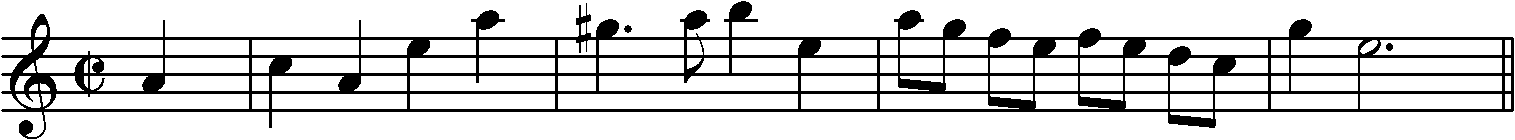
\includegraphics[width=140mm]{../img/primus-incipit-2}
    \verb`package_aa/000102439-1_1_1/000102439-1_1_1.png`
    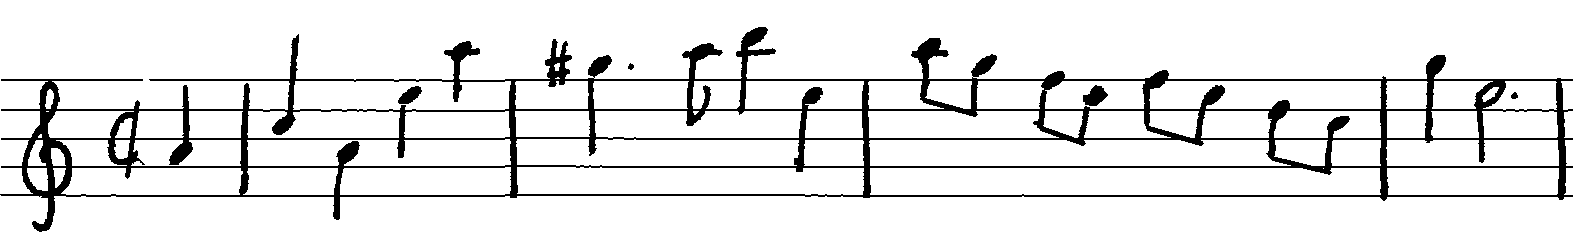
\includegraphics[width=140mm]{../img/primus-incipit-2-engraved}
    \verb`clef.G-2 time.C/ q-1 | q1 q-1 q3 q6 | #5 q5 * e6 q7 q3 |`
    \verb`e=6 =e5 e=4 =e3 e=4 =e3 e=2 =e1 | q5 h3 * |`
    \caption{An image engraved from an annotation taken from the PrIMuS dataset.}
    \label{fig6:PrimusIncipit}
\end{figure}

The advantage of this training data is that the music in it comes from the real world. This allows the model to pick up common patterns and possibly learn the language model.


\subsection{Synthetic Incipits}

The other option we have is to just simply randomize the training annotations, to create some synthetic data. We throw away the possibility of learning a language model, but we get a different benefit. We can artificially boost frequencies of tokens that appear lass frequently in the real world. This will cause the model to make fewer mistakes on uncommon symbols.

Randomization seems simple at first, but it can be done in many ways. At one extreme, we can simply randomly choose tokens from the vocabulary. This, however, produces sequences that cannot be rendered and are nonsensical. Beamed notes have to have a beginning and an end. We cannot have an unfinished or non-started beam. At another extreme, we can try to mimic the language model by using a lot of rules.

We opted for something in the middle. We make sure, that the synthetic annotation can be engraved, but we don't ensure anything more. Duration per measure is not correct, pitch is almost random, time signatures can be in the middle of a measure. The resulting image looks nothing like what we are used to seeing in sheet music. The code for generating synthetic annotations can be found in file \verb`app/`\allowbreak\verb`generate_`\allowbreak\verb`random_`\allowbreak\verb`annotation.py`.

\begin{figure}[h]
    \centering
    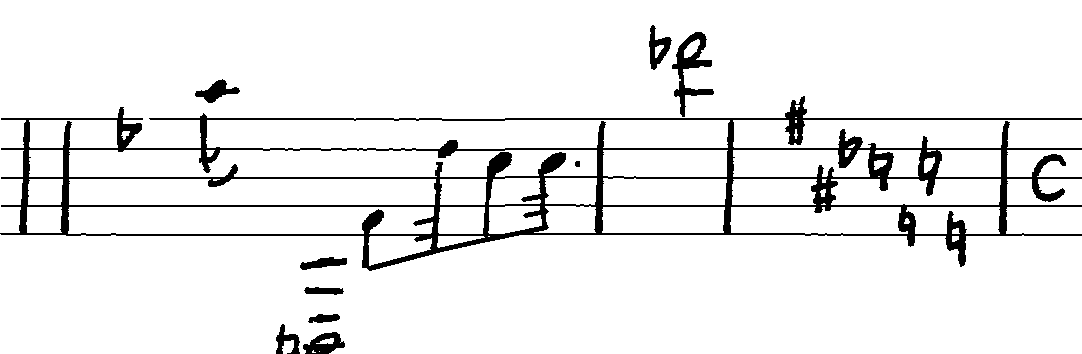
\includegraphics[width=140mm]{../img/synthetic-incipit}
    \verb`| | b3 s6 N-12 w-12 e=-3 =t=2 =e=1 =t1 * |`
    \verb`b9 h9 | #4 #-1 b2 N1 N-3 N1 N-4 | time.C`
    \caption{An image engraved from a synthetic annotation.}
    \label{fig6:SyntheticIncipit}
\end{figure}

We will compare these two approaches later in the experiments. It may come as a surprise, but the best approach will be to combine both synthetic and real-world data, effectively training on both.


\section{Evaluation Data}

When we faced the lack of training data, we resorted to data augmentation. We cannot do that for evaluation, because the evaluation data should be as close to the real-world as possible. Therefore using a well-established dataset it the only option.

By looking at the \emph{Collection of datasets for OMR} by Alexander Pacha (\cite{Pacha}) we can see that most existing datasets are for printed music. If we focus on the handwritten datasets, most of those contain only musical symbols, not entire staves. When we filter those out, what remains is CVC-MUSCIMA (\cite{CvcMuscima}), MUSCIMA++ (\cite{MuscimaPP}), and Baró Single Stave Dataset (\cite{HmrBaseline}). We are already familiar with the first two datasets since we used them for training. The last dataset is also derived from CVC-MUSCIMA and it is used in the paper for HMR baseline (\cite{HmrBaseline}). We will compare our results to the results in the paper in section~\ref{sec:ComparisonToOtherWorks}.

We decided to evaluate on a portion of the CVC-MUSCIMA dataset. Partly because it is the only dataset available for this purpose, partly because other people use it for evaluation as well. To learn more about the CVC-MUSCIMA dataset, see the section~\ref{sec:CvcMuscima}.

The fact that we devised custom encoding means we have to annotate the evaluation data manually. This is not very difficult, because the evaluation set need not be large. It also means the resulting annotations are of high quality and follow the rules of the Mashcima encoding.

We cannot use the entire CVC-MUSCIMA dataset for evaluation, because we already use it for training. Therefore we need to decide what portion is going to be used for evaluation. We definitely need to evaluate on data from different writers than those we train on. This is because seeing the specific writer's handwriting style might help the model score higher during evaluation. Avoiding specific music pages is not necessary since the data augmentation process completely destroys any rhythmic or melodic information. The Mashcima engraving system samples individual symbols, ignoring their placement relative to other symbols in the staff. So the primary concern is to separate writers used for evaluation.

There are additional criteria for selecting the evaluation writers. We want the writer selection to be diverse in terms of handwriting style. Some writers have very clean handwriting, some not so much. Noteheads can be little circles, ellipses, or even little dashes. Some writers have note stems slanted, some have straight, vertical stems. Also, the width and spacing of symbols differ.

We also want to evaluate on pages that are present in MUSCIMA++. This is because pages in MUSCIMA++ have a lot of additional information available and there exist detailed MusicXML transcriptions for them. Both of these facts may become useful in the future. Each writer has 20~music pages in CVC-MUSCIMA, but only 2 or 3 in MUSCIMA++. Additionally, not all pages can be represented in the Mashcima encoding (some are polyphonic or have multiple voices).

First, we sorted the 20~pages by how easily they can be encoded using Mashcima encoding (see table~\ref{tab6:MuscimaPagesByAnnotationEase}). This sorting is not perfect, the main goal is to separate pages that we cannot encode at all. Some symbols can be encoded, but since the engraving system cannot render them, they are considered slightly problematic. See the section on extending mashcima encoding (section~\ref{sec:RepresentationExtensibility}).

\begin{table}[h] \centering
\begin{tabular}{lll}
\toprule
\textbf{Page} & \textbf{Acceptable} & \textbf{Notes} \\
\midrule
03 & Yes       & perfect                                              \\
12 & Yes       & perfect                                              \\
02 & Yes       & trills, grace notes                                  \\
11 & Yes       & \verb`?` token                                       \\
09 & Yes       & \verb`?` token, fermata                              \\
05 & Yes       & trills                                               \\
01 & Yes       & triplets, fermata, rests in beamed groups            \\
13 & Yes       & \verb`?` token                                       \\
14 & Yes       & chord, triplets                                      \\
17 & Yes       & two staves with chords                               \\
15 & Yes       & rests in beamed groups                               \\
16 & Yes       & beamed notes with empty noteheads, accents           \\
06 & Not ideal & trills, many grace notes                             \\
04 & Not ideal & tenuto, triplets, nested slurs, bar repeat, fermata  \\
18 & Not ideal & two staves with chords                               \\
07 & No        & trills, many concurrent notes                        \\
08 & No        & grace notes, unsupported symbols, two voices in bass \\
20 & No        & chords in many places                                \\
10 & No        & chords                                               \\
19 & No        & multiple voices                                      \\
\bottomrule
\end{tabular}
\caption{All pages of CVC-MUSCIMA, sorted by how easily they can be represented using the Mashcima encoding.}
\label{tab6:MuscimaPagesByAnnotationEase}
\end{table}

Then we took all the acceptable pages and found all writers for those pages that are present in MUSCIMA++. We sorted those writers by the number of pages that satisfied our selection (see table~\ref{tab6:WritersConsideredForEvaluation}).

\begin{table}[h] \centering
\begin{tabular}{llll}
\toprule
\textbf{\# Pages} & \textbf{Writer} & \textbf{Handwriting style} &
\textbf{Selected} \\
\midrule
4 & 49 & worse, dash noteheads             & Yes \\
3 & 06 & nice, round noteheads             & No  \\
3 & 13 & regular, round noteheads          & Yes \\
3 & 20 & regular, dash noteheads           & Yes \\
3 & 27 & nice, round noteheads             & No  \\
3 & 34 & regular, round noteheads, slanted & Yes \\
3 & 41 & beautiful, round noteheads        & Yes \\
\bottomrule
\end{tabular}
\caption{Writers that were considered for the evaluation dataset.}
\label{tab6:WritersConsideredForEvaluation}
\end{table}

All the remaining writers had only two or fewer pages from the selection. We took 5~writers out of those 7~writers manually, to keep the handwriting diversity high.

Lastly, we wanted to compare our results with the results of \emph{From Optical Music Recognition to Handwritten Music Recognition: A baseline} (\cite{HmrBaseline}), so we added the writer~17. The final writer and page selection can be seen in the table \ref{tab6:EvaluationDataset}.

\begin{table}[h] \centering
\begin{tabular}{llll}
\toprule
\textbf{Writer} & \textbf{Pages} \\
\midrule
13 & 02, 03, 16     \\
17 & 01             \\
20 & 02, 03, 16     \\
34 & 02, 03, 16     \\
41 & 02, 03, 16     \\
49 & 03, 05, 09, 11 \\
\bottomrule
\end{tabular}
\caption{The evaluation dataset.}
\label{tab6:EvaluationDataset}
\end{table}

We end up with 6~writers, 17~pages (7~distinct), 115~staves, and over 5840~tokens. Annotations for these pages can be found in the file \verb`app/`\allowbreak\verb`mus`\allowbreak\verb`ci`\allowbreak\verb`ma_`\allowbreak\verb`annota`\allowbreak\verb`tions.py`. These annotations have been created by me --- the author of this thesis. Experience regarding the annotation process is described in the following section (section~\ref{sec:ManualAnnotationExperience}).

Lastly, we want to show a frequency table of the most common tokens in the evaluation dataset. The table contains generic variants of the tokens. A table containing common pitches is the very next table.

\begin{code}
table of generic tokens
\end{code}

\begin{code}
table of pitches
\end{code}

\newpage


\subsection{Manual Annotation Experience}
\label{sec:ManualAnnotationExperience}

Although the Mashcima encoding attempts to not be ambiguous, there were some places where we had to make some decisions regarding undefined situations. This section goes over these situations.

\paragraph{Page 1:} The last three measures contain nested slurs. These cannot be represented, so we chose to represent slur beginnings and slur endings as they appear on the page. One note cannot have two slur beginnings, so only one is annotated. The very last slur is maybe not a slur, but some pitch articulation symbol. We annotated it as a slur continuing onto the next staff.

\begin{figure}[h]
    \centering
    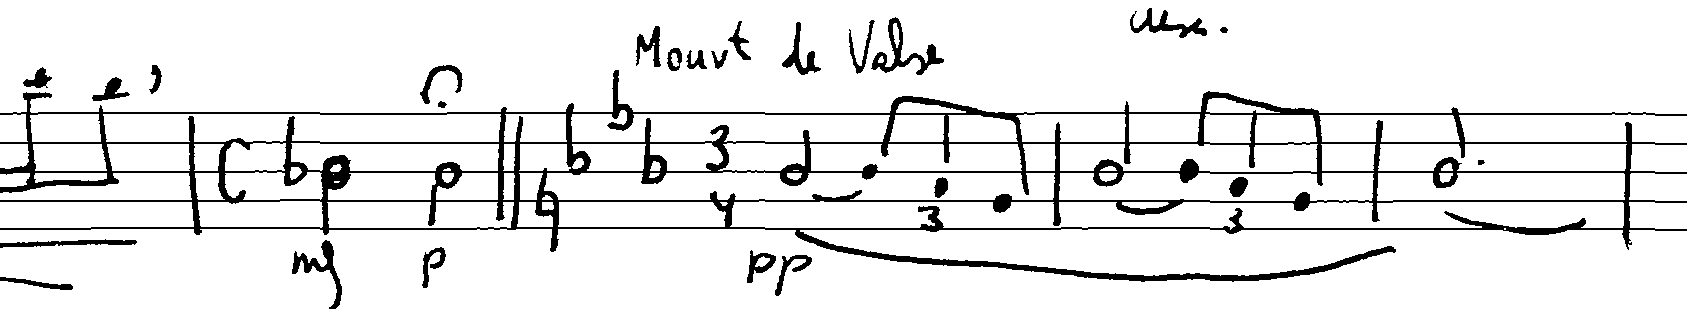
\includegraphics[width=140mm]{../img/ae-01}
    \verb`=s=8 =e7 | time.C b0 h0 fermata h0 | N-2 b1 b4 b0 time.3 time.4`
    \verb`h0 ( ) e=0 tuplet.3 =e=-1 =e-2 | h0 ( ) e=0 tuplet.3 =e=-1 =e-2`
    \verb`| ) h0 * ( ) |`
    \caption{Last three measures of page 01, writer 17.}
    \label{fig6:AnnotationExperience01}
\end{figure}

\paragraph{Page 2:} The last two staves contain three occurrences of grace notes. They look like regular notes but are smaller. Grace notes cannot be represented yet, so we replaced them with a \verb`?` token. We replaced the entire grace note group (two sixteenths with a slur) with a single \verb`?` token.

\begin{figure}[h]
    \centering
    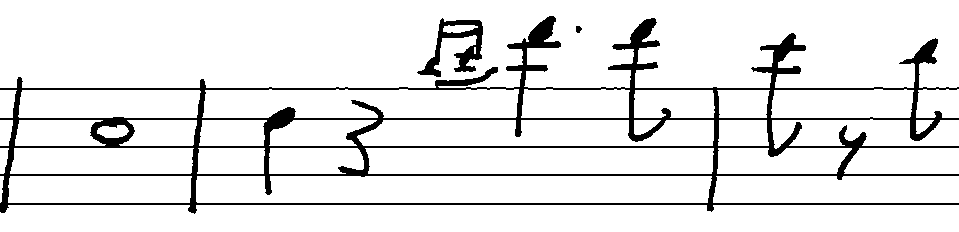
\includegraphics[width=80mm]{../img/ae-02}
    \verb`| w1 | q2 qr ? q9 * e9 | e8 er e7`
    \caption{Grace notes in page 02, writer 13.}
    \label{fig6:AnnotationExperience02}
\end{figure}

\paragraph{Page 9:} There are two measures with notes playing at the same time. The first three half notes are slightly offset, so we annotated them from left to right. The last two quarter notes are right above each other, so we replaced them with the \verb`?` token. We wanted to place at least one \verb`?` token inside the measure and then we tried to annotate the rest as good as we could. This way the measure is marked and can be repaired in the future.

\begin{figure}[h]
    \centering
    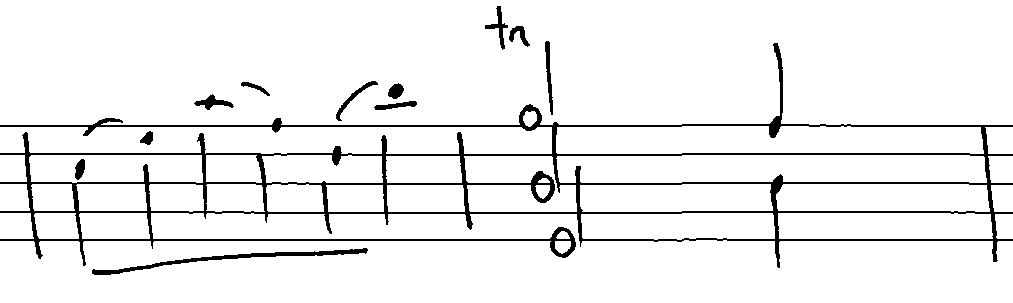
\includegraphics[width=90mm]{../img/ae-09}
    \verb`| e=1 ( ) =e=3 =e=6 ( ) =e=4 =e=2 ( ) =e7 | trill h7 h0 h-6 ? |`
    \caption{Simultaneous notes in page 09, writer 49.}
    \label{fig6:AnnotationExperience09}
\end{figure}

\paragraph{Page 11:} One measure has the same problem as page 9.

\paragraph{Page 16:} Third staff contains a bracket symbol in the key signature. The bracket symbol is completely ignored, but the clef and key signature are annotated as usual. The fifth staff contains double-beamed notes with empty noteheads. These are not sixteenth notes, but since they look so similar, we annotated them as such. These symbols are not very common and the trained model treated them as sixteenth notes as well, so we kept it that way.

\begin{figure}[h]
    \centering
    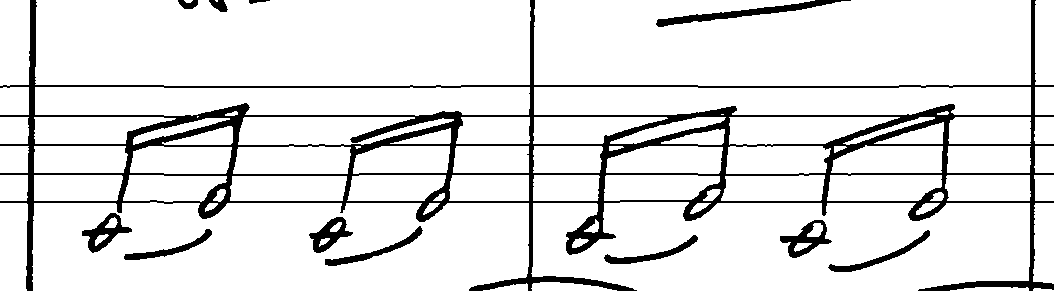
\includegraphics[width=100mm]{../img/ae-16}
    \verb`| s=-6 ( ) =s-4 s=-6 ( ) =s-4 | s=-6 ( ) =s-4 s=-6 ( ) =s-4 |`
    \caption{Beamed notes with empty noteheads in page 16, writer 34.}
    \label{fig6:AnnotationExperience16}
\end{figure}

Special thick barlines, double barlines, or barlines with braces at the beginning of a staff are all annotated as simple \verb`|` token. The only exception is repeat signs that do have their corresponding tokens.

There are many trills or accents throughout the pages. Those are not in the training data but can be represented, so they are annotated just as defined in the chapter on Mashcima encoding.


\section{Evaluation Metrics}

Now that we have a model producing some token sequences and we have our gold sequences, we need a way to measure the model performance. There are three goals for these measurements:

\begin{itemize}
\item Compare the model against itself to track improvements.
\item Get an overall idea of the model performance and compare it to other works.
\item Analyze model output to identify common mistakes it makes.
\end{itemize}

Looking at the work by Calvo-Zaragoza and Rizo (\cite{Primus}) or the HMR baseline article (\cite{HmrBaseline}) we can see, that the metric they use is \emph{Symbol Error Rate} (SER). This metric is also known as normalized Levenshtein distance or edit distance. The name Symbol Error Rate is used in contrast to Word Error Rate (WER) in the text recognition community. Since we don't work with text, we are left with the Symbol Error Rate only.

Regular Levenshtein distance (\cite{Levenshtein}) is defined as the minimum number of single-character edits that turn our prediction into the gold sequence. We don't work with strings, so we use tokens instead of characters. The basic edit operations are insertion, deletion, and substitution. The lower this number, the better. Zero means a perfect match.

This metric has to be normalized by the length of the gold sequence to allow for averaging over multiple values. Normalized Levehnstein distance produces a number that is typically between 0 and 1, where 0 means the sequences were predicted perfectly and 1 means the sequence is entirely wrong. The normalized distance can be greater than 1 when the predicted sequence is much longer than the gold one, but that happens only when the model is completely useless.

$$
SER = \text{LevNormalized} = \frac{\#\text{Insertions} + \#\text{Deletions} + \#\text{Substitutions}}{\text{GoldLength}}
$$

Since this metric is also used by other works, we will use it for comparison against these works.

When training, we will use the edit distance function implemented in the Tensorflow\footnote{\href{http://tensorflow.org/}{http://tensorflow.org/}} library. Although it is claimed to be the normalized Levenshtein distance, the implementation is different from the one used during evaluation. Therefore these two values should not be compared directly. The training edit distance is only meant for tracking the learning process a determining the stopping condition.


\subsection{Understanding Model Mistakes}
\label{sec:UnderstandingModelMistakes}

We would like to get an idea of the kind of mistakes our trained model makes. The chapter \ref{chap:MusicRepresentation} talks about the Mashcima encoding and how it can represent symbols that it cannot yet represent (by the \verb`?` token). Having this \verb`?` token in the gold data creates an ever-present mistake, that increases our error rate. We would like to get an estimate of how much of the overall error is contributed by such symbols. Also, note that \verb`?` is not the only token the model cannot produce. Some symbols cannot be engraved yet, like trills, accents, or fermatas. Being able to measure the error these tokens contribute would give us an idea of how much the model could improve if we implemented these symbols in the engraving system.

During the evaluation, we will take the prediction and remove certain tokens from it. These same tokens will be removed from the gold sequence as well. We will compute the error of these simplified sequences. Comparing this error to the baseline error should tell us how much the removed tokens contribute to the baseline error.

The metric used for computing this error will be the Levenshtein distance but normalized by the number of \emph{important tokens} in the gold sequence. An \emph{important token} is a token that will never be removed. It can be altered, but not removed. This will make sure the normalization term stays constant over all the possible transformations and thus all the error values should be comparable.

\emph{Important tokens} are notes, rests, barlines, clefs, accidentals, and other similar tokens. What remains as non-important is slurs, ornaments, and the \verb`?` token. The specific list of important tokens can be found in the file \verb`app/`\allowbreak\verb`voca`\allowbreak\verb`bula`\allowbreak\verb`ry.py`. We will call this metric \emph{Important Token Error Rate} (ITER). Remember that this metric should not be used for comparison against other models using different encodings. It is purely to get an idea of what mistakes contribute to the Symbol Error Rate.

With this metric we propose a set of transformation functions that progressively simplify the sequences:

\begin{itemize}
\item \verb`ITER_RAW` \\ No transformation is applied, corresponds to SER, but normalized by the number of important tokens.
\item \verb`ITER_TRAINED` \\ Tokens that the model hasn't seen during training are removed (\verb`?` token, trills, fermatas, etc.).
\item \verb`ITER_SLURLESS` \\ Like the above, but slurs are removed as well (\verb`(`, \verb`)`).
\item \verb`ITER_ORNAMENTLESS` \\ Like the above, but most of the non-important attachments are removed (trill, accent, staccato, fermata, ...). What has to remain are accidentals and duration dots. Those are important for correct pitch and rhythm.
\item \verb`ITER_PITCHLESS` \\ Like the above, but all pitch information is removed by converting all tokens to their generic variant.
\end{itemize}

Each metric builds on the previous one, further simplifying the sequences. This means the error rate should decrease as we go down. The amount by which it decreases can tell us how much the given transformation affected the error, therefore how much the removed tokens contributed to the error rate.

Also please understand, that all these errors are computed on a single trained model. The gold sequence is modified during evaluation. Not during training. We are trying to understand a specific model we have.


\section{Architecture, Training, and Evaluation}
\label{sec:ArchitectureTrainingEvaluation}

In chapter \ref{chap:DeepNeuralNetwork} we provided a short introduction to deep neural networks and described the RCNN architecture. We will use this architecture in the following experiments. Here is the list of layers, used in the neural network:

\begin{code}
tabulka s vrstvama sítě a jejich parametrama
\end{code}

The Mashcima engraving system works with images at the resolution of the CVC-MUSCIMA dataset. Image of an engraved staff is about 400 pixels in height and the width varies from 500 to over 2000 pixels. The neural network however requires the input image to be exactly 64 pixels in height. The image will be scaled down because of this while preserving its aspect ratio.

There will be two datasets used for training. One for the actual training --- a \emph{training dataset} and one for validation --- a \emph{validation dataset} (or \emph{dev dataset}). The training dataset is fed into the model in batches and each batch is used to perform an update of the learned parameters of the model. This process is called stochastic gradient descent (\cite{Goodfellow-et-al-2016}). Using the entire training dataset once is called \emph{one epoch}. The validation dataset will be used after each epoch to estimate the true performance of the model (to estimate the generalization error).

Learned parameters will be updated by the adaptive learning rate optimizer (Adam) (\cite{AdamOptimizer}), that comes with Tensorflow\footnote{\href{http://tensorflow.org/}{http://tensorflow.org/}}, with the default parameters:

\begin{table}[h] \centering
\begin{tabular}{l@{\hspace{1.5cm}}l}
\toprule
\textbf{Parameter} & \textbf{Value} \\
\midrule
Learning rate & 0.001     \\
$\beta_1$     & 0.9       \\
$\beta_2$     & 0.999     \\
$\varepsilon$ & $10^{-8}$ \\
\bottomrule
\end{tabular}
\caption{Adam optimizer parameters.}
\label{tab6:AdamParameters}
\end{table}

We have not tried to fine-tune these parameters or any other hyperparameters. Our goal was to try training on engraved handwritten images and see whether this approach is even feasible. Tuning hyperparameters is one of the places where our approach can be improved in the future.

The training will run for a given number of epochs. In each epoch, an average symbol error rate on the validation dataset is recorded. The final trained model is the model, that had the lowest validation symbol error rate, during the whole training. If the number of epochs trained is sufficiently high, this method should return the model at the point, where the generalization error began to rise. Also, note that the symbol error rate here is the edit distance function from Tensorflow. It is a different implementation of SER than the one used for evaluation.

During the evaluation, the beam search decoding algorithm is used with a beamwidth of 100 (\cite{CtcBeamSearch}). There are two additional steps performed after that. Firstly the produced token sequence is repaired. This means the rules regarding beamed notes are checked and corrected and attachment tokens are sorted properly. This repairing process is relatively simple and completely rule-based. For the details see the \verb`repair_`\allowbreak\verb`annotation` function inside \verb`app/`\allowbreak\verb`voca`\allowbreak\verb`bula`\allowbreak\verb`ry.py`. After the repairing process, leading and trailing barlines are stripped from both gold data and the prediction. This is because barlines at the beginning and at the end of staff convey no additional meaning. It is analogous to trimming whitespace characters around a sentence. Barlines with repeat signs are not stripped away since they are important.


\section{Experiments}

In the section on training data (section~\ref{sec:TrainingData}) we hypothesized some differences between training on PrIMuS incipits and synthetic data. The main idea is that training on PrIMuS incipits should allow the model to learn the language model. More generally training on real-wold music samples should help the model, since it will be evaluated on real-world music in the CVC-MUSCIMA dataset. Training on synthetic data should allow the model to learn complicated combinations of symbols, that are not as common in real-world music.

To test this hypothesis we propose a set of four experiments (table~\ref{tab6:ExperimentData}).

\begin{table}[h] \centering
\begin{tabular}{lll}
\toprule
\textbf{Experiment} & \textbf{Training data} & \textbf{Validation data} \\
\midrule
1 & 63 000 PrIMuS                   & 1 000 PrIMuS    \\
2 & 63 000 synthetic                & 1 000 synthetic \\
3 & 31 500 PrIMuS, 31 500 synthetic & 1 000 PrIMuS    \\
4 & 63 000 PrIMuS, 63 000 synthetic & 1 000 PrIMuS    \\
\bottomrule
\end{tabular}
\caption{Training data (number of incipits) for the proposed experiments.}
\label{tab6:ExperimentData}
\end{table}

The first experiment trains a model on real-world incipits, second uses synthetic incipits and the third one combines both approaches in a 1:1 ratio. The last experiment validates on real-world incipits since the evaluation will also be performed on real-world music. The second experiment validates on synthetic incipits because we wanted to simulate a scenario where we don't have access to real-world incipits. The fourth experiment is the same as the third one, only utilizing the whole PrIMuS dataset as is available to us.

We trained each experiment for 20~epochs (except for the fourth that has been trained for only 10~epochs) and took the model with the lowest edit distance, averaged over the validation dataset.

\begin{code}
graphs of the validation & training edit distances from the tensorboard
\end{code}


\section{Results}
\label{sec:Results}

The table~\ref{tab6:ExperimentSER} shows the resulting symbol error rates, averaged over the entire validation dataset.

\begin{table}[h] \centering
\begin{tabular}{ll}
\toprule
\textbf{Experiment} & \textbf{Symbol error rate} \\
\midrule
1 & 0.34 \\
2 & 0.28 \\
3 & 0.26 \\
\textbf{4} & \textbf{0.25} \\
\bottomrule
\end{tabular}
\caption{Symbol error rates on the evaluation dataset for each experiment.}
\label{tab6:ExperimentSER}
\end{table}

It seems that training on synthetic data is better than training on real-world data. But looking at experiment~3, we see that the best approach is to combine both approaches. Synthetic data is probably better than real-world data simply because all the tokens are represented equally. The discussion on the language model is more complicated and is explored in a separate section (section~\ref{sec:LanguageModel}). The experiment~4 is slightly better than the experiment~3 because it has twice as much data to train on.

In section~\ref{sec:UnderstandingModelMistakes} we proposed a set of metrics, intended to give us insight into the mistakes the model makes. Table~\ref{tab6:ExperimentITER} shows these ITER metrics for each experiment.

\begin{table}[h] \centering
\begin{tabular}{l@{\hspace{1.5cm}}lllll}
\toprule
\mc{} & \multicolumn{5}{c}{\textbf{ITER Metrics}} \\
\pulrad{\textbf{Experiment}} & \footnotesize{\verb`RAW`}
& \footnotesize{\verb`TRAINED`} & \footnotesize{\verb`SLURLESS`}
& \footnotesize{\verb`ORNAMENTLESS`} & \footnotesize{\verb`PITCHLESS`} \\
\midrule
1 & 0.44 & 0.42 & 0.30 & 0.26 & 0.21 \\
2 & 0.37 & 0.34 & 0.28 & 0.25 & 0.17 \\
3 & 0.34 & 0.32 & 0.24 & 0.21 & 0.16 \\
3 & 0.33 & 0.31 & 0.23 & 0.21 & 0.16 \\
4 & 0.33 & 0.31 & 0.23 & 0.21 & 0.16 \\
\bottomrule
\end{tabular}
\caption{ITER metrics (section~\ref{sec:UnderstandingModelMistakes}) on the evaluation dataset for each experiment.}
\label{tab6:ExperimentITER}
\end{table}

When we compare the \verb`ITER_RAW`, \verb`ITER_TRAINED`, and \verb`ITER_SLURLES`, we can see that reducing our focus to only trained tokens helps slightly, although it's not as big of an impact as we expected. A considerably larger difference happens when we remove slur tokens. This confirms, what can be seen by looking manually at the predictions the model makes. There are a lot of mistakes related to slur classification. This might be caused by the fact that the engraving system does not capture all the variability that exists in the real world with regards to slur engraving.

In a previous section on evaluation (section~\ref{sec:ArchitectureTrainingEvaluation}) we mentioned, that the prediction, before being evaluated, is repaired by a few rules (attachment sorting, barline trimming). The table~\ref{tab6:RepairComparison} shows how much impact the repair has on the error rate.

\begin{table}[h] \centering
\begin{tabular}{lll}
\toprule
\textbf{Experiment} & \textbf{Raw SER} & \textbf{Repaired prediction SER} \\
\midrule
1 & 0.34 & 0.34 \\
2 & 0.28 & 0.28 \\
3 & 0.26 & 0.26 \\
4 & 0.25 & 0.25 \\
\bottomrule
\end{tabular}
\caption{Comparison of repaired and non-repaired predictions.}
\label{tab6:RepairComparison}
\end{table}

You can see, that there's almost no difference. The repairs were indeed disabled, it's just that the performance difference was so minor, that the resulting average is the same.

Now that we know the experiment~4 performed the best, we will take a closer look at it. The table~\ref{tab6:MetricsForEachPage} shows metrics for each evaluation page (averaged over all staves in that page).

\begin{table}[h] \centering
\begin{tabular}{llllllll}
\toprule
\mc{} & \mc{} & \mc{} & \multicolumn{5}{c}{\textbf{ITER Metrics}} \\
\pulrad{\textbf{Page}} & \pulrad{\textbf{Writer}} & \pulrad{\textbf{SER}}
& \footnotesize{\verb`RAW`}
& \footnotesize{\verb`TRAINED`} & \footnotesize{\verb`SLURLESS`}
& \footnotesize{\verb`ORNAMENTLESS`} & \footnotesize{\verb`PITCHLESS`} \\
\midrule
02 & 13 & 0.16 & 0.18 & 0.17 & 0.17 & 0.14 & 0.12 \\
03 & 13 & 0.12 & 0.13 & 0.13 & 0.07 & 0.06 & 0.04 \\
16 & 13 & 0.30 & 0.42 & 0.40 & 0.33 & 0.27 & 0.21 \\
01 & 17 & 0.28 & 0.37 & 0.31 & 0.26 & 0.23 & 0.16 \\
02 & 20 & 0.26 & 0.32 & 0.30 & 0.27 & 0.24 & 0.14 \\
03 & 20 & 0.11 & 0.12 & 0.12 & 0.07 & 0.06 & 0.05 \\
16 & 20 & 0.32 & 0.48 & 0.44 & 0.27 & 0.22 & 0.15 \\
02 & 34 & 0.28 & 0.34 & 0.32 & 0.29 & 0.24 & 0.15 \\
03 & 34 & 0.06 & 0.07 & 0.07 & 0.03 & 0.03 & 0.02 \\
16 & 34 & 0.34 & 0.49 & 0.47 & 0.35 & 0.29 & 0.19 \\
02 & 41 & 0.23 & 0.27 & 0.25 & 0.24 & 0.22 & 0.14 \\
03 & 41 & 0.14 & 0.16 & 0.16 & 0.07 & 0.07 & 0.06 \\
16 & 41 & 0.28 & 0.41 & 0.37 & 0.29 & 0.23 & 0.14 \\
03 & 49 & 0.29 & 0.33 & 0.33 & 0.24 & 0.24 & 0.21 \\
05 & 49 & 0.24 & 0.26 & 0.25 & 0.21 & 0.21 & 0.18 \\
09 & 49 & 0.42 & 0.61 & 0.59 & 0.36 & 0.35 & 0.33 \\
11 & 49 & 0.50 & 0.67 & 0.67 & 0.50 & 0.48 & 0.44 \\
\bottomrule
\end{tabular}
\caption{All metrics for each page in the evaluation dataset.}
\label{tab6:MetricsForEachPage}
\end{table}

We can average the results for each writer and compare them to the style of their handwriting (table~\ref{tab6:SerAverageForWriters}).

\begin{table}[h] \centering
\begin{tabular}{lll}
\toprule
\textbf{Writer} & \textbf{SER} & \textbf{Handwriting style} \\
\midrule
13 & 0.19 & regular, round noteheads          \\
41 & 0.22 & beautiful, round noteheads        \\
34 & 0.23 & regular, round noteheads, slanted \\
20 & 0.23 & regular, dash noteheads           \\
17 & 0.28 & regular, round noteheads          \\
49 & 0.36 & worse, dash noteheads             \\
\bottomrule
\end{tabular}
\caption{Symbol error rates averaged for each writer and handwriting style of each writer.}
\label{tab6:SerAverageForWriters}
\end{table}

The first four writers are very much comparable, but the writer~49 has the worst handwriting of all the writers and he ended up last, as expected.

Similarly, we can average over each page and compare it to the annotation difficulty notes we took eralier (table~\ref{tab6:SerAverageForPages}).

\begin{table}[h] \centering
\begin{tabular}{lll}
\toprule
\textbf{Page} & \textbf{SER} & \textbf{Notes} \\
\midrule
03 & 0.14 & perfect                                    \\
02 & 0.23 & trills, grace notes                        \\
05 & 0.24 & trills                                     \\
01 & 0.28 & triplets, fermata, rests in beamed groups  \\
16 & 0.31 & beamed notes with empty noteheads, accents \\
09 & 0.42 & \verb`?` token, fermata                    \\
11 & 0.50 & \verb`?` token                             \\
\bottomrule
\end{tabular}
\caption{Symbol error rates averaged for each page and annotation notes for each page.}
\label{tab6:SerAverageForPages}
\end{table}

Pages 9 and 11 ended up last because they are only present for writer~49, who ended up as the worst writer. Page~3 is very interesting. It is the only page, that can be fully encoded using Mashcima encoding and all the symbols it contains can be engraved using the Mashcima engraving system. It is, however, also the simplest page in that it does not contain any complicated expressions and contains only a few slurs. This is supported by the fact that page~5 ended up with an also very low error and page~5 is very much comparable in its layout and complexity to page~3.

\newpage


\subsection{Language Model}
\label{sec:LanguageModel}

Symbol error rates on the evaluation dataset for each experiment. When comparing the results of training on real-world data vs. synthetic data, it is strange that pure synthetic data outperform purely real-world data. But it probably has to do with the fact, that the synthetic dataset is balanced with respect to the individual output class abundance. The learned language model of real-world data helps the first experiment, but it's not nearly enough to beat the benefits of a balanced dataset for the second experiment.

This idea is supported by the fact that the third experiment beats both of the first two. It can benefit from both a balanced dataset and from learning a language model.

Experiment 3 does indeed learn a basic language model. When I was annotating the evaluation dataset I used a trained model from experiment 3 and I noticed, that if often made mistakes in beamed note groups. Especially for the writer 49. It classified the first note of a beamed group as a quarter note. But then it (incorrectly) classified the second note as a beam start note, even though it can be easily seen the beam runs to both sides of the note. It preferred a well-formed beam, rather than the correct token. This property can be learned even from synthetic data since they contain well-formed beams only.

\begin{code}
image of a misclassified first eight as quarter note
predicted: ...
gold: ...
expected without language model: ...
\end{code}

Then there are a couple of places where it correctly predicts key signature, even though an accidental is misplaced by the writer. In a key signature, the number and type of accidentals
uniquely identify, what pitches those accidentals have. For example, when there's only a single sharp, it always corresponds to an \verb`F#` note. Combining this with a specific clef gives us a correct position for the sharp.

\begin{code}
find image of that place with comparison of individual experiment predictions
(01 correct (hopefully), 02 wrong (hopefully), 03 correct)
\end{code}


\section{Comparison to Other Works}
\label{sec:ComparisonToOtherWorks}

We wanted to make a comparison against the HMR baseline article (\cite{HmrBaseline}) because our evaluation datasets overlap. Specifically, we share page~3 for writer~13 and page~1 for writer~17. We both use the symbol error rate metric, although many differences need to be addressed. Their model classifies rhythm and pitch separately, so both error rates are provided. There is also a combined error rate that treats the output symbols similar to our Mashcima encoding --- having pitch and rhythm in one token (this number should be analogous to ours). The last column shows our error rate, given by the experiment~4.

\begin{table}[h] \centering
\begin{tabular}{llcccr}
\toprule
\mc{} & \mc{} & \multicolumn{3}{c}{\textbf{HMR baseline SERs}} & \mc{} \\
\pulrad{\textbf{Page}} & \pulrad{\textbf{Writer \qquad}}
& \mc{Rhythm} & \mc{Pitch} & \mc{Combined}
& \multicolumn{1}{r}{\pulrad{\textbf{\qquad Our SER}}} \\
\midrule
1 & 17 & 0.528 & 0.349 & 0.592 & 0.28 \\
3 & 13 & 0.226 & 0.175 & 0.270 & 0.12 \\
\bottomrule
\end{tabular}
\caption{Comparison of our model from experiment 4 to the model proposed by the HMR baseline article (\cite{HmrBaseline}).}
\label{tab6:ComparisonToHmrBaseline}
\end{table}

You can see, that our model has a much smaller error rate, but we have to consider this result carefully. Their model does not use the CTC loss and the output encoding is very different. While our model might output a sequence of length 50, their model produces a sequence of the same length as the width of the input image, which is in the order of hundreds to a thousand sequence items. Also, their encoding requires perfect alignment. If the model transitions between output classes at slightly different time-steps then the gold data, it produces a lot of error, even though when collapsed, the resulting sequence is the same. And given the temporal resolution, this might contribute a lot.

A more fair comparison would be a qualitative one. Luckily the paper provides a qualitative comparison of one staff from page~3 of their model against a commercial software called PhotoScore\footnote{\href{https://www.neuratron.com/photoscore.htm}{https://www.neuratron.com/photoscore.htm}}. We can add a prediction by our model and compare all three (see figure~\ref{fig6:HmrBaselineComparison03}). Note that the image has been produced by manually engraving the predicted Mashcima annotation.

\begin{figure}[p]
    \centering

    \setlength{\unitlength}{1.0cm}
    \begin{picture}(14,7.5)
        %\thicklines
        %\put(0,0){\line(1,0){14}}
        %\put(0,0){\line(0, 1){7.5}}

        \put(0,2){
            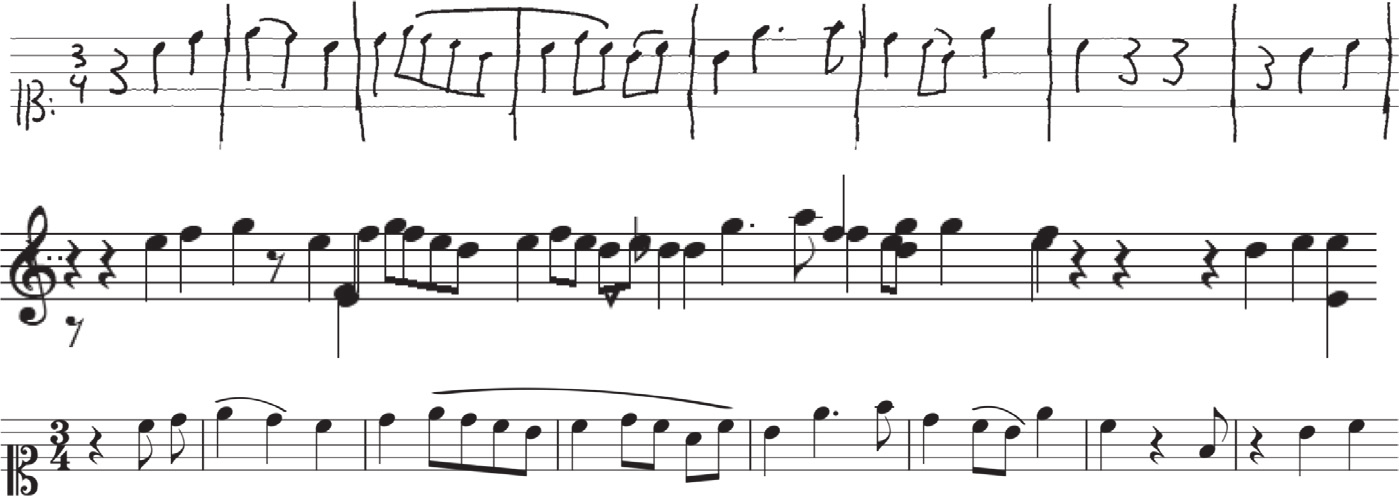
\includegraphics[width=138mm]{../img/hmr-baseline-comparison-their-03}
        }
        \put(0,0){
            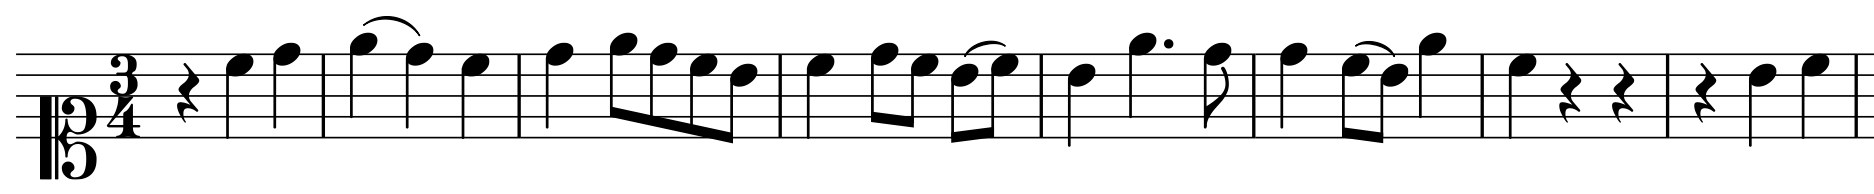
\includegraphics[width=138mm]{../img/hmr-baseline-comparison-our-03}
        }

        \put(0,1.3){\footnotesize \texttt{Our result:}}
        \put(0,3.0){\footnotesize \texttt{HMR baseline:}}
        \put(0,5.0){\footnotesize \texttt{PhotoScore:}}
        \put(0,7.0){\footnotesize \texttt{Input:}}
    \end{picture}
    \verb`clef.C-4 time.3 time.4 qr q3 q4 | q5 ( ) q4 q3 |`
    \verb`q4 e=5 =e=4 =e=3 =e2 | q3 e=4 ) =e3 e=2 ( ) =e3 |`
    \verb`q2 q5 * e4 | q4 e=3 ( ) =e2 q5 | q3 qr qr | qr q2 q3`
    \caption{Comparison of our results to the HMR baseline article on page 03, writer 13.}
    \label{fig6:HmrBaselineComparison03}
    \medskip
    \small
    The upper part (first three staves) are taken from the HMR baseline article (\cite{HmrBaseline}). The first staff is the input image from CVC-MUSCIMA, page 03, writer 13. The second staff is what produced the commercial software PhotoScore. The third staff is what the HMR baseline article achieved and the last staff is what our model returned, together with the Mashcima annotation. The image was created from the annotation by hand using MuseScore (\href{https://musescore.org/}{https://musescore.org/}).
\end{figure}

You can see, that the difference is not as pronounced, although this staff is one of the simpler ones. There is, however, also a qualitative comparison on a staff from page 1 (see figure~\ref{fig6:HmrBaselineComparison01}).

\begin{figure}[p]
    \centering

    \setlength{\unitlength}{1.0cm}
    \begin{picture}(14,6.5)
        %\thicklines
        %\put(0,0){\line(1,0){14}}
        %\put(0,0){\line(0, 1){6.5}}

        \put(0,1.6){
            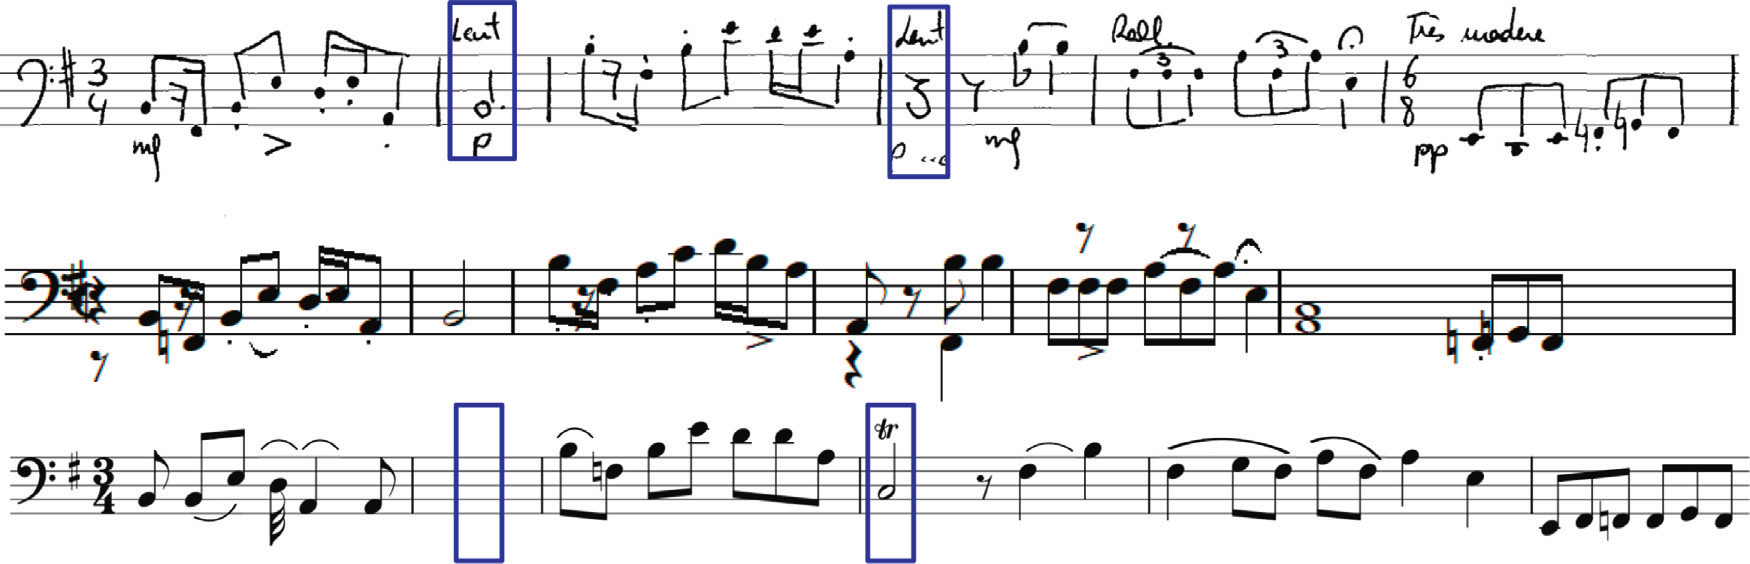
\includegraphics[width=138mm]{../img/hmr-baseline-comparison-their-01}
        }
        \put(0,0){
            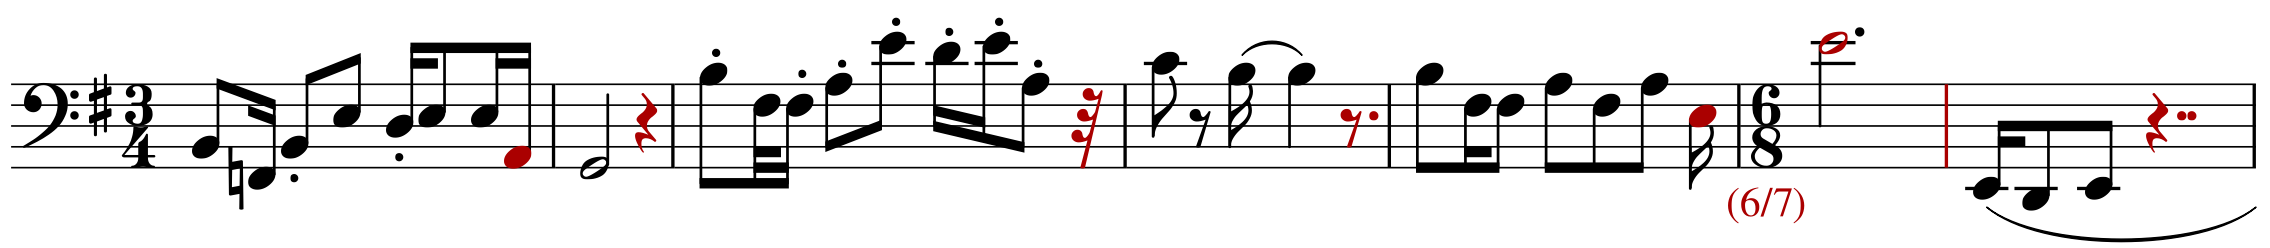
\includegraphics[width=138mm]{../img/hmr-baseline-comparison-our-01}
        }

        \put(0,1.3){\footnotesize \texttt{Our result:}}
        \put(0,2.8){\footnotesize \texttt{HMR baseline:}}
        \put(0,4.3){\footnotesize \texttt{PhotoScore:}}
        \put(0,6.0){\footnotesize \texttt{Input:}}
    \end{picture}
    \verb`clef.F2 #2 time.3 time.4 e=-2 N-5 =s-5 e=-2 . =e1 s=0 . =e=1`
    \verb`=s=1 =e-3 | h-4 | e=5 . =t=2 =s2 . e=4 . =e8 . s=7 . =s=8 .`
    \verb`=e4 . | e6 er s5 ( ) q5 | e=5 =s=2 ) =e2 e=4 =e=2 =e4 e1 |`
    \verb` time.6 time.7 w8 * s=-6 ( =e=-7 =e-6 |`
    \caption{Comparison of our results to the HMR baseline article on page 01, writer 17.}
    \label{fig6:HmrBaselineComparison01}
    \medskip
    \small
    The upper part (first three staves) are taken from the HMR baseline article (\cite{HmrBaseline}). The first staff is the input image from CVC-MUSCIMA, page 01, writer 17. The second staff is what produced the commercial software PhotoScore. The third staff is what the HMR baseline article achieved and the last staff is what our model returned, together with the Mashcima annotation. The image was created from the annotation by hand using MuseScore (\href{https://musescore.org/}{https://musescore.org/}).
    The blue boxes are part of the original image and they show difficulties with recognizing symbols placed above each other. The red symbols in the last staff show errors introduced during manual engraving. MuseScore requires rhythm to be correct. For the actual output of our model refer to the Mashcima annotation below the staff.
\end{figure}

Both models make a lot of mistakes on this more difficult input so it isn't easy to tell which one is better. What we can conclude is that their performance is actually very comparable.

It should also be noted, that each model uses a different resolution for input images. The model from HMR article normalizes to a height of 100 pixels, whereas ours normalizes to only 64 pixels. This might be a disadvantage for us. Also, our model cannot read chords by design, but theirs can. This might very well be required for some task and it would make our model unusable. Their model can also detect the presence of dynamics and text.

\section{Evaluating on Printed PrIMuS Incipits}

We also wanted to try, how would our model perform on printed music. Models by other people are often pre-trained on printed music and then fine-tuned on handwritten images via transfer learning. Ours is different in that it has never seen an image of printed music. We already have code for parsing PrIMuS dataset and since the dataset contains images as well, we will use those. We just slightly preprocessed the images --- inverted them, normalized, and slightly scaled down to have dimensions comparable to what our model trained on. We used the model from experiment 4 since it performed the best. The evaluation was performed on 100 incipits that the model hasn't seen during training and these are the results:

\begin{table}[h] \centering
\begin{tabular}{l@{\hspace{1.5cm}}lllll}
\toprule
\mc{} & \multicolumn{5}{c}{\textbf{ITER Metrics}} \\
\pulrad{\textbf{SER}}
& \footnotesize{\verb`RAW`}
& \footnotesize{\verb`TRAINED`} & \footnotesize{\verb`SLURLESS`}
& \footnotesize{\verb`ORNAMENTLESS`} & \footnotesize{\verb`PITCHLESS`} \\
\midrule
0.61 & 0.64 & 0.64 & 0.60 & 0.59 & 0.56 \\
\bottomrule
\end{tabular}
\caption{All metrics, evaluated on printed primus incipits. Our model wasn't trained on printed music so the performance suffers.}
\label{tab6:MetricsOverPrintedPrimus}
\end{table}

You can see, that the performance is not very impressive. We did expect the error rate to be high, but not that high. Although, it is understandable because the printed music is very different from the handwritten. It would be interesting to also train on printed images in the future. This error rate would go down, but maybe the CVC-MUSCIMA error rate would go down as well.

\begin{figure}[h]
    \centering
    \verb`package_ab/211002723-1_1_1/211002723-1_1_1.agnostic`
    \\
    \medskip
    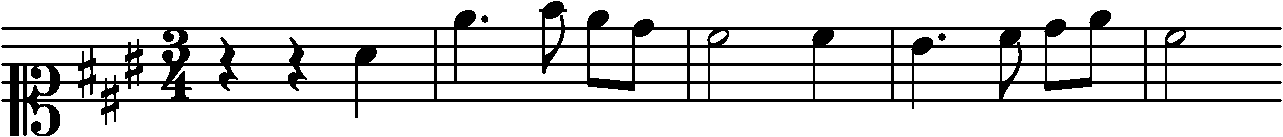
\includegraphics[width=140mm]{../img/evaluation-on-printed}
    \textbf{Gold:}
    \verb`clef.C-4 #-1 #-4 #0 time.3 time.4 qr qr q1 |`
    \verb`q5 * e6 e=5 =e4 | h3 q3 | q2 . e3 e=4 =e5 | h3`
    \\
    \medskip
    \textbf{Prediction:}
    \verb`clef.C-4 #-1 #-4 #0 time.8 time.2 qr q1 |`
    \verb`q5 * s7 s=5 =e4 | h3 q3 | h2 ( time.9 time.4 e=4 =e5 | h3`
    \\
    \medskip
    \textbf{SER:}
    \verb`0.35`
    \caption{Evaluation on printed PrIMuS incipits.}
    \label{fig6:EvaluatinoOnPrinted}
\end{figure}

Also, note that \verb`ITER_RAW` and \verb`ITER_TRAINED` have the same value. This is expected because we filter out incipits that cannot be engraved by Mashcima.

\chapter{Conclusion and Future Work}
\label{chap:ConclusionAndFutureWork}

Handwritten text recognition is an interesting and unique field of research. We can see it is mainly held back by the lack of training data. It shows the fact, that we were able to achieve state-of-the-art results by writing a simple engraving system. The MUSCIMA++ dataset is a step in the right direction. It provides excessive amounts of information about the music from which we can extract any specific encoding (be it with a little bit of work). It has to be done this way because commonly used encodings (MusicXML, MEI, MIDI) express the semantic meaning of the music and lack visual information, whereas any lower-level encodings depend too much on the chosen model architecture and so cannot be used to compare different models. The MUSCIMA++ encodes music on a low level, from which high-level information can be extracted.

End-to-end solutions are powerful since they can learn intermediate features by themselves. The problem is that training an end-to-end model is much more challenging because it requires a lot more data. The MUSCIMA++ dataset has barely enough data to learn symbol classification and segmentation. When we want the model to extract pitch information about notes, the dataset becomes far too small. It is understandable because annotating data at such a high level of precision is very expensive.

Our Mashcima engraving system cannot yet engrave many symbols (chords, trills, repeats, dynamics, text) and this functionality could easily be added. We think that scaling the engraving system now would be a far too early optimization. The system relies heavily on the Mashcima encoding. This is ok for the task we tackled in this thesis --- it was ideal for our model architecture. But should this engraving system be extended in the future, there are many more fundamental places it can change:

\begin{itemize}
    \item What should the input look like? This will depend a lot on the final architecture because the input has to be capable of expressing everything the system can engrave. This would be an API at the source code level for which adapters from other formats (MusicXML) could be added.

    \item What format and resolution the output image has? Currently, we produced only binary images that are already very refined. We could generate RGB images that look like photos or scans. We could even leave raster graphics and produce a vector output.

    \item We could provide more information in addition to the output image. We could produce the annotation XML file that MUSCIMA++ uses. Suddenly our system would be useful for symbol segmentation as well as end-to-end learning.

    \item The way engraving is implemented could be different. Currently, the system moves around sprites. But when it tries to render slurs and beams, sprites become inconvenient. Maybe we could draw everything as curved lines, simulating the pen on the paper (we need it for slurs and beams anyway).
\end{itemize}

There is also a lot of discussions to be had about the model architecture. It seems that each architecture has pros and cons and there is not yet a fit-all solution. Most of these differences have been mentioned many times throughout the thesis. We think that an engraving system capable of producing high-quality training data would make for a valuable common ground on which different HMR approaches could be directly compared.

The goal of this thesis was to create a model capable of recognizing handwritten music. The goal was fulfilled and we also created an interesting engraving system that could be further explored in the future. Our model does not produce MusicXML as stated in the assignment but Mashcima encoding instead. Conversion from Mashcima to MusicXML was not implemented because we wanted to focus on the model and the engraving system instead.


%%% Bibliography
%%% Bibliography (literature used as a source)
%%%
%%% We employ bibTeX to construct the bibliography. It processes
%%% citations in the text (e.g., the \cite{...} macro) and looks up
%%% relevant entries in the bibliography.bib file.
%%%
%%% The \bibliographystyle command selects, which style will be used
%%% for references from the text. The argument in curly brackets is
%%% the name of the corresponding style file (*.bst). Both styles
%%% mentioned in this template are included in LaTeX distributions.

\bibliographystyle{plainnat}    %% Author (year)
% \bibliographystyle{unsrt}     %% [number]

\renewcommand{\bibname}{Bibliography}

%%% Generate the bibliography. Beware that if you cited no works,
%%% the empty list will be omitted completely.

\bibliography{bibliography}

%%% If case you prefer to write the bibliography manually (without bibTeX),
%%% you can use the following. Please follow the ISO 690 standard and
%%% citation conventions of your field of research.

% \begin{thebibliography}{99}
%
% \bibitem{lamport94}
%   {\sc Lamport,} Leslie.
%   \emph{\LaTeX: A Document Preparation System}.
%   2nd edition.
%   Massachusetts: Addison Wesley, 1994.
%   ISBN 0-201-52983-1.
%
% \end{thebibliography}


%%% Figures used in the thesis (consider if this is needed)
\listoffigures

%%% Tables used in the thesis (consider if this is needed)
%%% In mathematical theses, it could be better to move the list of tables to the beginning of the thesis.
\listoftables
\XXX{In mathematical theses, it could be better to move the list of tables to the beginning of the thesis.}

%%% Abbreviations used in the thesis, if any, including their explanation
%%% In mathematical theses, it could be better to move the list of abbreviations to the beginning of the thesis.
\chapwithtoc{List of Abbreviations}
\XXX{In mathematical theses, it could be better to move the list of abbreviations to the beginning of the thesis.}

%% PHDONLY
%%% Doctoral theses must contain a list of author's publications
\chapwithtoc{List of publications}
\XXX{Doctoral theses must contain a list of author's publications.}
%% ONLYPHD

%%% Attachments to the bachelor thesis, if any. Each attachment must be
%%% referred to at least once from the text of the thesis. Attachments
%%% are numbered.
%%%
%%% The printed version should preferably contain attachments, which can be
%%% read (additional tables and charts, supplementary text, examples of
%%% program output, etc.). The electronic version is more suited for attachments
%%% which will likely be used in an electronic form rather than read (program
%%% source code, data files, interactive charts, etc.). Electronic attachments
%%% should be uploaded to SIS and optionally also included in the thesis on a~CD/DVD.
%%% Allowed file formats are specified in provision of the rector no. 72/2017.
\appendix
\chapter{Attachments}
\XXX{Attachments to the bachelor thesis, if any. Each attachment must be referred to at least once from the text of the thesis. Attachments are numbered.}
\XXX{The printed version should preferably contain attachments, which can be read (additional tables and charts, supplementary text, examples of program output, etc.). The electronic version is more suited for attachments which will likely be used in an electronic form rather than read (program source code, data files, interactive charts, etc.). Electronic attachments should be uploaded to SIS and optionally also included in the thesis on a~CD/DVD. Allowed file formats are specified in provision of the rector no. 72/2017.}

\section{First Attachment}

\openright
\end{document}
